\documentclass[12pt,a4paper]{report}

\usepackage{styles/dolgozat}

\usepackage{listings}

\renewcommand{\lstlistingname}{Programkód}

\usepackage{styles/cpp}
\usepackage{styles/python}
\usepackage{styles/java}


\usepackage{hyperref}
% cleveref csomag és beállításai -- az egyetlen, amit a hyperref után kell betölteni!
\usepackage{styles/refs}

\begin{document}

\pagestyle{empty}
\pagenumbering{gobble}

\begin{titlepage}
\centering
% A Miskolci Egyetem címere
\vspace*{2cm}
\huge\textsc{\textbf{Szakdolgozat}}\\[1cm]
%\vspace*{1cm}

\includegraphics[width=4.8cm, height=4cm,keepaspectratio]{images/me_logo.png}\\
\textbf{\textsc{Miskolci Egyetem}}

\vspace*{2cm}

% A szakdolgozat címe, akár több sorban is
{\LARGE\textbf{Régiség webáruház készítése}}

\vspace*{2cm}
% A hallgató neve, évfolyam, szak(ok), a konzulens(ek) neve
\large
\textbf{Készítette:}\\[0.8ex]
Bártfai Bálint\\[0.8ex]
Programtervező informatikus

\vspace*{0.5cm}
\textbf{Témavezető:}\\[0.8ex]
Dr.Agárdi Anita

\vfill

% Keltezés: Hely, év
\large
\textbf{\textsc{Miskolc, 2023}}

\end{titlepage}
%Feladatkiiras
\noindent
\textsc{\textbf{Miskolci Egyetem}}\\
Gépészmérnöki és Informatikai Kar\\
Alkalmazott Matematikai Intézeti Tanszék\hspace*{4cm}\hfil \textbf{Szám:}

\vspace{0.5cm}
\begin{center}
\large\textsc{\textbf{Szakdolgozat Feladat}}
\end{center}
\vspace{0.5cm}

Bártfai Bálint (NWTTCA) BSc programtervező informatikus jelölt részére.

\bigskip
\noindent\textbf{A szakdolgozat tárgyköre:} Webfejlesztés

\bigskip
\noindent\textbf{A szakdolgozat címe:} Régiség webáruhás készítése

\bigskip
\noindent\textbf{A feladat részletezése:}

\medskip

A szakdolgozat egy modern webáruház készítéséről szól, melyet angular, node.js és mongoDB használatával hozok létre. A webáruházat használó egyének képesek a termékek közti keresésre szűrők segítségével és a kiválasztott termék megvásárlására. A felhasználók képesek regisztrációra és ezután bejelentkezésre is. A normál felhasználói joggal rendelkezők csak vásárlásra képesek, az adminisztrátor joggal rendelkező emberek pedig képesek a termékek hozzáadására és levételére is. A dolgozat célja a webáruház teljeskörű bemutatása.

\medskip


\vfill

\noindent\textbf{Témavezető:} Dr.Agárdi Anita, egyetemi adjunktus

% \noindent\textbf{Konzulens(ek):} (akkor kötelezõ, ha a témavezetõ nem valamelyik matematikai tanszékrõl való; de persze lehet egyébként is)\newline

\bigskip
\noindent\textbf{A feladat kiadásának ideje:} 2022.02.21.

\noindent\textbf{A feladat beadásának határideje:} 2023.11.17.

\vspace{1.5cm}

\hfill\makebox[6cm]{\dotfill}

\hfill\makebox[6cm]{szakfelelős}

\clearpage

\vspace*{1cm}  
\begin{center}
\large\textsc{\textbf{Eredetiségi Nyilatkozat}}
\end{center}
\vspace*{2cm}  

Alulírott \textbf{Bártfai Bálint}; Neptun-kód: \texttt{NWTTCA} a Miskolci Egyetem Gépészmérnöki és Informatikai Karának végzős Programtervező informatikus szakos hallgatója ezennel büntetőjogi és fegyelmi felelősségem tudatában nyilatkozom és aláírásommal igazolom, hogy \textit{Régiség webáruhás készítése}
című szakdolgozatom saját, önálló munkám; az abban hivatkozott szakirodalom
felhasználása a forráskezelés szabályai szerint történt.

\medskip
Tudomásul veszem, hogy szakdolgozat esetén plágiumnak számít:
\begin{itemize}
\item szószerinti idézet közlése idézőjel és hivatkozás megjelölése nélkül;
\item tartalmi idézet hivatkozás megjelölése nélkül;
\item más publikált gondolatainak saját gondolatként való feltüntetése.
\end{itemize}

Alulírott kijelentem, hogy a plágium fogalmát megismertem, és tudomásul veszem, hogy
plágium esetén szakdolgozatom visszautasításra kerül.

\vspace*{3cm}

\noindent Miskolc, \makebox[2cm]{\dotfill}. év \makebox[2cm]{\dotfill}. hó \makebox[2cm]{\dotfill}. nap

\vspace*{3cm}

\hfill\makebox[6cm]{\dotfill}

\hfill\makebox[6cm]{Hallgató}



\clearpage

\newcommand{\ki}{témavezető(k)}
\newsavebox{\alairas}
\begin{lrbox}{\alairas}
\begin{tabular}{c@{\hspace{2cm}}c}
\makebox[4cm]{\dotfill} & \makebox[5cm]{\dotfill} \\
dátum & \ki \\
\end{tabular}
\end{lrbox}
\newcommand{\dotline}{\makebox[5cm]{\dotfill}}
\newcommand{\shortdotline}{\makebox[3.5cm]{\dotfill}}

\noindent 1.
\begin{tabular}[t]{cl}
\multirow{2}{*}{A szakdolgozat feladat módosítása}
&szükséges (módosítás külön lapon) \\
& nem szükséges\\[1ex]
\end{tabular}

\begin{center}
\usebox{\alairas}
\end{center}

\smallskip

\noindent 2. A feladat kidolgozását ellenőriztem:

\begin{center}
\begin{tabular}{c@{\hspace*{2cm}}c}
témavezető (dátum, aláírás): & konzulens (dátum, aláírás):\\
\dotline & \dotline \\
\dotline & \dotline \\
\dotline & \dotline 
\end{tabular}
\end{center}

\smallskip

\noindent 3. A szakdolgozat beadható:

\begin{center}
\usebox{\alairas}
\end{center}

\noindent 4.
\begin{tabular}[t]{@{}l@{\hspace*{1mm}}l@{\hspace*{1mm}}l}
A szakdolgozat & \shortdotline & szövegoldalt\\
              & \shortdotline & program protokollt (listát, felhasználói leírást)\\
              & \shortdotline & elektronikus adathordozót (részletezve)\\
              & \shortdotline \\
              & \shortdotline & egyéb mellékletet (részletezve)\\
              & \shortdotline 
\end{tabular}
\newline tartalmaz.

\begin{center}
\usebox{\alairas}
\end{center}

\noindent 5.
\begin{tabular}[t]{ll}
\multirow{2}{*}{A szakdolgozat bírálatra} & bocsátható\\
& nem bocsátható\\
\end{tabular}

\smallskip

\noindent A bíráló neve: \makebox[8cm]{\dotfill}

\renewcommand{\ki}{szakfelelős}
\begin{center}
\begin{tabular}{c@{\hspace{2cm}}c}
\makebox[4cm]{\dotfill} & \makebox[5cm]{\dotfill} \\
dátum & \ki \\
\end{tabular}
\end{center}

\noindent 6.
\begin{tabular}[t]{lll}
A szakdolgozat osztályzata \\
& a témavezető javaslata: & \makebox[2.5cm]{\dotfill} \\
& a bíráló javaslata: & \makebox[2.5cm]{\dotfill} \\
& a szakdolgozat végleges eredménye: & \makebox[2.5cm]{\dotfill}
\end{tabular}

\bigskip\bigskip

\noindent Miskolc, \makebox[4cm]{\dotfill} \hfill \makebox[8cm]{\dotfill} 

\hfill \makebox[8cm]{a Záróvizsga Bizottság Elnöke} 


\tableofcontents

\clearpage
\pagenumbering{arabic}
\pagestyle{fancy}

\chapter{Bevezetés}

A mai rohanó világunkban az informatika egyre nagyobb teret hódít magának, ez nagyban megkönnyíti az életünket. Az egyik ilyen, gyakran használt informatikai fejlesztés az internetes vásárlás. Az ehhez használt webáruházak hasznosak az üzletek számára, mivel így olyan vásárlókat is elérhetnek, akik különben a nagy távolság miatt nem őket választanák. A webáruházak segítségével a vásárlást kényelmesen, otthonról is meg lehet ejteni, egy-egy termék beszerzéséhez nem szükséges fizikálisan ingázni a boltok között, ezáltal nő a vásárlói élmény. 

A webáruházi vásárlás mára már annyira népszerű lett, hogy egyes üzletláncok applikációin keresztül már a hétvégi bevásárlást is el tudjuk intézni, amivel éves szinten több órát tudunk magunknak megspórolni.

A webáruházat vásárlók széles köre használja, emiatt szükséges a felület könnyű kezelhetősége és átláthatósága. Mivel a webáruházakra nagy kereslet van, az üzletek nem engedhetik meg maguknak, hogy az oldaluk igénytelen legyen. Hiszen hiába használható jól az oldal, ha nem esztétikus, nem fogja a vevők érdeklődését felkelteni. Emellett a fejlesztőknek arra is oda kell figyelniük, hogy a felhasználók többféle webböngészőt is használni fognak - ezek közül a legismertebbek a Google Chrome, Microsoft Edge, Opera, Mozilla Firefox, Safari - tehát gondoskodniuk kell arról, hogy a weboldal minél több böngészőben használható legyen. Egy sikeres webáruház létrehozásához azonban nem elég a széles termékkínálat és az esztétikus megjelenés. Oda kell figyelnünk, hogy a vásárlók képesek legyenek megtalálni a keresett terméket. Ezt kategóriák és szűrők használatával kell segíteni, így a felhasználó képes lesz céltudatosan vásárolni, amivel időt fog megspórolni. Ezáltal, ha az adott oldalt kielégíti a vásárlók igényeit, akkor a későbbiekben is vissza fognak ide térni, vásárolni.

A jövőben remélhetőleg tengernyi felhasználó fogja használni webáruházunk, akik temérdek rendelést fognak leadni, így lesznek olyan termékek, amelyek elfogynak, emellett érkezhetnek új termékek is. Ezek kezelésére szükség lesz adminisztrátorokra. Ezért biztosítani kell plusz funkciókat, amelyeket a normál felhasználók, vásárlók nem használhatnak. Így két fajta felhasználó lesz: a vásárló és az adminisztrátor.

A fentebbiekből is látható, hogy egy modern, megfelelően működő, a vásárlói igényeket kielégítő webáruház létrehozása komoly kihívás elé állítja a fejlesztőket. 

Szakdolgozatom célja egy olyan régiségekkel, azon belül főként numizmatikával foglalkozó webáruház létrehozása, amely a fentebb leírt követelményeknek megfelel. Azért ezt a témát választottam, mert tanulmányaim során a webes alkalmazások készítése keltette fel leginkább az érdeklődésem, emellett magam is gyűjtök régiségeket, így számos alkalommal vásároltam webáruházakból, mégsem találtam olyan oldalt, amely teljes mértékig kielégítette volna felé támasztott szükségleteimet. Mindegyik oldalnak számos hibája volt, gyakran a termékek közötti szűrési lehetőség nem volt elég alapos vagy nem is volt szűrési lehetőségem, így megnehezítették vásárlásomat, kevésbé tudtam céltudatosan választani. 

\chapter{Technológiák}
\overfullrule=0pt
\section{HTML}

Egy weboldal létrehozásához elengedhetetlen, hogy a fejlesztőnek legyenek ismeretei az HTML-ről \cite{1} másnéven HyperText Markup Languageről, magyarul Hiperszöveges Jelölőnyelvről. Ez tulajdonképpen egy leíró nyelv, melyet weboldalak létrehozásához hoztak létre, annak érdekében, hogy ne legyen szükség pluginek telepítésére.

Egy HTML három fő részből áll össze. Az első a Dokumentum Típus Definíciója röviden DTD, ez a dokumentum legelején található. Ez határozza meg, hogy az adott dokumentum HTML lesz. Nincsen záró tagja. Például: <!DOCKTYPE html>. 

További példa még a <HTML></HTML>. Ezen nyitó, valamint zár tag közé fog kerülni az egész oldalunk. Ez közvetlen a <!DOCKTYPE html> elem után következik.

A második a fejléc, mely tartalmazza a technikai és a dokumentációs adatokat. Ezeket a felhasználók nem látják, tehát a böngésző nem jeleníti meg. Ilyen például a <title></title> amely meghatározza a HTML oldal nevét. Ezt a böngésző innen, a fejlécből olvas ki. Jelölése: <head></head>

A harmadik fő rész közvetlenül a fejléc után következik, ez a HTML törzse, mely azokat az információkat tartalmazza, amelyet a böngésző meg fog jeleníteni a felhasználók számára. Jelölése:<body></body>


\section{JavaScript}

Egy weboldal létrehozásának elengedhetetlen eleme a Javascript \cite{2}. Az évek során ez lett a világon egyik leggyakrabban használt programozási nyelv. Főként platformfüggetlen alkalmazások létrehozására használják, tehát az adott alkalmazást bármelyik böngészőből képesek futtatni. Ez egy kliens oldali programozási nyelv, tehát csak azokat a dolgokat tudjuk vele elintézni, amelyek a kliens, a felhasználó oldalán történnek. Ennek segítségével képes a JavaScript felismerni a HTML oldalakba beágyazott utasításokat, ezáltal képes a felhasználói eseményekre reagálni, például egérklikkelés vagy form beküldés.

 Emellett ez egy objektum orientált, prototípus alapú szkriptnyelv, ami kifejezetten weboldalakhoz lett kifejlesztve. Futtatásához a fejlesztőnek nincs szüksége külön fordítóra, magában a böngészőben tudja futtatni. Ez annak köszönhető, hogy a webböngészőkben van beépített JavaScript-motor. Ezen alkalmazásokat viszont nem csak böngészőből tudjuk futtatni, hanem azon kívül is, például a node.js-sel, ami több operációs rendszerrel is kompatibilis.
 
A JavaScript egy laza típusú nyelv. Tehát deklarálásnál nem kell megadni az adott változó adattípusát, mivel a JavaScript az átkonvertálást automatikusan elvégzi nekünk. Ezért például előfordulhat, hogy az adott változó egyszer egy integer, utána pedig egy string lesz.


\section{CSS}

Egy weboldal létrehozásánál a kinézetére is oda kell figyelni, ebben nyújt segítséget a CSS \cite{3}, angolul Cascading Style Sheet. Ez egy stílus leíró nyelv, amely a HTML típusú dokumentumok kialakítását adja meg. Ezzel nem csak HTML típusú, de még az XML típusú dokumentumok kinézetén is tudunk változtatni. A CSS-sel meg lehet adni a lapok színét/hátterét, betűtípusát, elrendezését és még sok más, megjelenéshez vonatkozó elemet meg lehet változtatni. Ennek segítségével el lehet különíteni a HTML struktúráját a HTML kinézetétől. Ez több szempontból is hasznos: CSS használatával növekszik a weblapunk használhatósága, jobban áttekinthető lesz; sokkal rugalmasabb lesz a megjelenítése, kisebb képernyő használatakor sem fog szétesni az oldal. A felsoroltak ugyanúgy érvényesek XML dokumentumnál is, mivel ennek szintén részletesen állítható a stílusa, tehát be tudjuk ezen is állítani a színét, elhelyezkedését és betűtípusát is a webböngészőben.

Az adott elemek stílusát a szektorok kiválasztásával tudjuk megadni.

Minden elemre a * szimbólumot használjuk. Ez az egész HTML-re vonatkozik. 

Tudunk szűrni az elem neve alapján - például lehet ’p’ vagy ’div’ -, ekkor a megadott típusú elemből a változtatások az összes elemre vonatkozni fognak. 

Emellett tudunk szűrni leszármazottak alapján is, például, ha egy ’div’-ben van egy lista, aminek a jelölése ’li’ ekkor a ’li’ a ’div’ elem része lesz, így a ’div li’ szelektorral tudunk rá hivatkozni. Tehát a ’div’-en belül tartózkodó ’li’-re fog csak vonatkozni.

Képesek vagyunk még hivatkozni elemekre class vagy id alapján is. Class esetén a .class, Id esetén pedig \#id-val tudjuk használni a szelektort.

A CSS-ben rendelkezésre állnak pszeudo osztályok is, amelyekkel műveletekhez lehet stílusokat hozzárendelni. Például megváltozik az elem színe, ha felé visszük az egeret.

Az CSS-t többféleképpen lehet a HTML-hez hozzá csatolni. Két típusa létezik a külső és a belső CSS.

Össze lehet kapcsolni a HTML fájlt egy külső CSS dokumentummal. Ez a leggyakrabban használt, mivel ilyenkor a CSS fájl teljes mértékben külön áll a HTML fájltól. Így a kódunk sokkal átláthatóbb lesz. Ezáltal ezt a külső fájlt több oldalhoz is tudjuk használni így, ha a weboldalunk több HTML-ből áll, akkor azokat egységesíteni tudjuk, így még esztétikusabb lesz.\\

\textbf{Ennek szintaktikája a következő:}
\begin{itemize}
    \item[]<link ref=stylesheet type=”text/css” href=”CSS.ELÉRÉSI\_ÚTVONAL”> 
\end{itemize}


Ezt a kódsort a fejlécbe kell elhelyezni.

Másik módszer, amivel külön álló fájlként használjuk a CSS-t amikor stíluslapként importáljuk be. Ezt ugyan úgy a fejlécben kell megadni.\\

\textbf{Ennek a szintaktikája:}
\begin{itemize}
    \item[]@import url(ELÉRÉSI\_ÚTVONAL) 
\end{itemize}


A belső CSS-t már kevésbé használják a fejlesztők, de azért néha erre is szükség van. Az egyik ilyen módszer, amikor közvetlen az elem kezdő címkéjében helyezzük el a stílust. Ennek előnye, hogy gyorsan létrehozható, nem kell hozzá a fejlécben külön részt vagy külön CSS fájlt létrehozni. Hátránya viszont, hogy ez csak egyetlen elemre vonatkozik, így ezt nem lehet több elem módosítására használni.

A következő belső CSS-t már lehet alkalmazni több elemre is. Ez sokkal jobban hasonlít arra, mint amikor egy külső fájlból dolgozunk, csak itt a fejlécben ’style’ tagok közé helyezzük el a CSS-t. Előnye, hogy nem kell új fájlt létrehoznunk, viszont ekkor sokkal hosszabb és kevésbé átlátható lesz a kódunk, ami nehezíti a későbbi fejlesztést. Emellett figyelembe kell vennünk, több HTML esetén minden oldalhoz külön meg kell írni a CSS-t és nem lehet egységesíteni úgy, mint amikor külön fájlban van.

\cite{4} Mivel a CSS megfelelő beállítása sok időt elvessz a fejlesztőktől ezért CSS keretrendszereket hoztak létre, amiket már a natív CSS helyett szívesebben alkalmaznak. Ennek köszönhetően jóval hatékonyabbak lesznek és jóval nagyobb termelékenységet tesz lehetővé a CSS keretrendszer. Elsősorban reszponzív weblapok készítéséhez lett tervezve, amely asztali számítógépen, laptopon és okostelefonon lehetővé tesz jól megjelenő weboldalak létrehozását. Napjainkra már több ilyen keretrendszer is létrejött a fejlesztők és tervezők örömére. Ezeknek különböző képességekkel és rugalmassággal rendelkeznek. Népszerűségüket annak köszönhetik, hogy egyszerűek és könnyen tanulhatóak. Szinte már nem lehet olyan weboldalt találni, aminél ne használnák ennek több oka is van. Ezek az okok a következőek: Időt spórol meg mivel a feladatokat automatizálja, stabil munkafelületet biztosít, segítségével a mobil barát felülettel rendelkezik és támogatja a böngészők közti problémák megoldását.

\section{Angular}
\subsection{Bevezetés az Angularba}
Az Angular \cite{5} egy TypeScript és komponens alapú keretrendszer, amelyet első sorban egy oldalas (single page) webes alkalmazások fejlesztésére hoztak létre a Google TypeScript nyelven. Szakdolgozatom elkészítéséhez azért ezt választottam, mert ezt a keretrendszert világszerte rengeteg fejlesztő használja, ez az egyik legelterjedtebb keretrendszer, így nagy tudásbázis áll rendelkezésemre, minden felmerülő problémámra könnyen és gyorsan tudok megoldást találni.

Az Angular a webes alkalmazások készítéséhez HTML-t és TypeScript-et használ. A lényeges és az opcionális funkciókat könyvtárakkal valósítja meg, ezeket a fejlesztő importálja az alkalmazásba. Az Angular alapvető elemei a komponensek, ezek NgModul-okba szerveződnek. Ez az NgModule kódokat funkcionális halmazokba gyűjti össze, ezek fogják a későbbiekben meghatározni az alkalmazásunkat. Egy Angular alkalmazásnak mindig van egy gyökérmodulja, amely lehetővé teszi a bootstrapping-et. A komponensek ” view”-okat, magyarul nézeteket definiálnak. Ezek olyan képernyőelemek halmazai, amelyeket az Angular a program logikájának és adatainak ismerete alapján képes módosítani. A komponensek szolgáltatásokat használnak, viszont ezek a szolgáltatások közvetlen nem kapcsolódnak a nézetekhez. Azonban beilleszthetőek a komponensekbe és ennek segítségével a programunk moduláris, újra használható és sokkal hatékonyabb lesz. A modulok, komponensek és a szolgáltatások dekorátorokat alkalmaznak. Ezek jelzik az Angular-nak, hogy miként használhatják őket.

A komponens osztály metaadatai tulajdonképpen egy sablont alkotnak, amely HTML részekhez kapcsolódik, ez lehetővé teszi az Angular számára, hogy a megjelenésük előtt módosítsa a HTML elemeket.

A szolgáltató osztályok lehetővé teszik a z Angular-nak a függőség beillesztését a komponensek részére.
\subsection{Modulok}
Több NgModule áll rendelkezésre az Angular számára, amelyek kiegészítik a JavaScript modulokat. Ez a modul annak érdekében, hogy a modulok egységet alkossanak, komponensekhez társíthat kódot, például a szolgáltatásokat. Mint fentebb is említettem, egy Angular alkalmazásnak kizárólag egyetlen egy gyökérmodulja van, ez pedig egy NgModule osztály. Ezt az osztályt egységesen AppModule-nak nevezik, ez pedig az app.modul.ts fájlban helyezkedik el. Az alkalmazást ezzel a gyökér NgModule bootstrappingjével indítjuk el. Egy kisebb alkalmazásnak általában csak egy NgModule-ja van, az alkalmazások nagy részének viszont jóval több funckiómodulja van. A gyökér NgModule-t azért hívják így, mert a hierarchiában tetszőleges mélységig tartalmazhat gyermekmodulokat. Az NgModul-ok képesek funkciókat importálni más modulokból és saját funkcióikat exportálni más NgModul-ok számára, akárcsak a JavaScript modulok. A kód különálló modulokra való bontása megkönnyíti a fejlesztést, az átláthatóságot, valamint az újrahasználhatóságot. Ezáltal, ha valamit ki akarunk cserélni az alkalmazásunkban, nem kell az egész kódon módosítani, elég az adott modult megváltoztatni vagy kicserélni. Emellett még egy nagy előnye van, a ’lazy loading’, ami azt jelenti, hogy a modulokat külön is be lehet tölteni. Ezzel lecsökkenti a betölteni kívánt kódok mennyiségét, amivel a fejlesztők rengeteg időt meg tudnak spórolni a fejlesztés során.
\subsection{Komponensek}
A komponens a képernyő nézetét vezérli. Ez a következőkből áll: egy TypeScript osztályból, amely az alkalmazás logikáját és adatait definiálja; egy CSS stílusból; és egy HTML-ből, ami összekapcsolja az elemeket. Egy Angular alkalmazásnak mindig van minimum egy darab komponense, ez a gyökérkomponens. Ez a komponens köti össze a komponenshiearchiát a dokumentum objektum modell-el (DOM).

A komponens az az osztály, amely közvetlen egy @Component() dekorátor alatt helyezkedik el, ez meghatározza az adott osztály metaadatait. A metaadatok megmondják az Angular-nak, honnan kell megszereznie a nézet megjelenítéséhez és elkészítéséhez létfontosságú elemeket.

\subsection{Sablonok, direktívák és adatköztés}
A sablon hasonlít egy szokásos HTML fájlhoz, viszont ez tartalmaz Angular sablon szintaxist is, amely módosítja a HTML-t még a megjelenés előtt. A sablon képes használni adatkötést, ami pedig összeköti a DOM-ot, az alkalmazás adatait és direktívákat, ezek összessége biztosítja a programlogikát. 

Az adatkötésnek két fajtája van: az eseménykötés és a tulajdonságkötés. 

Eseménykötés: lehetővé teszi, hogy a felhasználói bemenetre reagáljon az alkalmazás az adatainak frissítésével.

Tulajdonságkötés: lehetővé teszi, hogy a HTML-be kiszámított értéket helyezhessünk be az alkalmazás adataiból.

Keretrendszer nélkül a fejlesztőnek kéne az adatelemeket feltöltenie a HTML-re a felhasználói válaszok és érték frissítések megváltoztatásáért. Viszont ezek megírása nagyon hosszadalmas munka, amiben rengeteg hibát lehet véteni. Emellett az Angular támogatja a két irányú adatkötést, tehát változások nem csak a DOM-ban történnek meg, hanem a programadatban is. Ez azért lehetséges, mert a sablon részei összehangolhatóak a komponens részeivel, utána csak meg kell mondani az Angular-nak, hogyan kapcsolja össze a két részt.

Az adatkapcsolat nem csak a sablon és komponens közti kommunikációban vállal nagy szerepet, hanem a szülő-gyermek komponensek közti kommunikációban is.

A sablonok képesek ” pipe”-okat használni. Ezek a @Pipe dekorátorral ellátott osztályok egy függvényt definiálnak, amely a beérkező értékeket kimeneti értékké alakítja át a megjelenítéshez, ezzel nagymértékben növelve a felhasználói élményt.

\subsection{Szolgáltatások és függősége beillesztése}
A szolgáltatások (service) magukba foglalnak minden értéket, funkciót és tulajdonságot, amire az alkalmazásnak szüksége van. A szolgáltatás osztályokat az @Injectable() dekorátor előzi meg, ennek segítségével lehetséges más függőségeket beilleszteni az osztályainkba. Ezek az osztályok olyan adatok és logikák számára vannak fenntartva, melyeket megosztunk a komponensek között úgy, hogy közben a nézetekhez nem kapcsolódnak.

A függőségi beillesztésnek köszönhetően a komponens osztályok megmaradnak hatékonynak és tömörnek, ezek csak továbbítják a feladatokat a szolgáltatásoknak. Ez a függőségi beillesztés (DI) az Angular azon része, mely hozzáférést biztosít a szolgáltatásokhoz és erőforrásokhoz a komponensek részére.

A komponensek szolgáltatásokat használnak azokra a feladatokra, melyek nem érintik az alkalmazás logikáját vagy a nézetet. Egy ilyen szolgáltatást több komponens is használhat a feladata elvégzésére.

\subsection{Átirányítás (Routing)}
Az Angularban a Router NgModul egy szolgáltatást biztosít, amely lehetővé teszi navigációs útvonal létrehozását az alkalmazás különböző állapotai és a nézet hierarchia között.
\subsection{Navigációs konvenciók}
Amikor a felhasználó a címsorba beír egy URL-t akkor az az adott oldalra navigálja.

Az oldalakon található linkre kattintva a böngésző a megadott oldalra navigálja a felhasználót.

A böngészőben található „vissza”, illetve „tovább” gombra kattintva a böngésző az előzmények alapján a megfelelő oldalra navigál. Ez azért lehetséges, mert a böngésző naplózza az előzményeket.

Az átirányítás az URL-szerű útvonalakat nem oldalakként tárolja el, hanem nézetekhez rendeli.


\section{TypeScipt}
A TypeScript-et \cite{6} a Microsoft hozta létre, mint a JavaScript szuperkészlete, ezért a már meglévő JavaScript alkalmazások is használhatóak TypeScript alkalmazásként. A szuperkészlet azt jelenti, hogy használni tudja a JavaScript már meglévő funkcióit, struktúrákat és hozzá tud adni bizonyos funkciókat, amelyek korábban nem voltak a JavaScript részei. Viszont a böngészők csak a JavaScript-et értik, ezért a TypeScript-be írt alkalmazásokat először le kell fordítania a fejlesztőnek, és ezzel JavaScript-be kell konvertálni.

A TypeScript-ben már deklarálni kell adattípust. Így már a programunk képes kiértékelni, hogy az adatstruktúrához rendelt értékek megegyeznek-e a deklarált adattípussal. Az esetben, ha nem egyezik meg, akkor a programunk hibára fut. Ez azért is nagyon jó, mert így a programon dolgozó fejlesztők hamarabb észreveszik a hibákat.

A TypeScript elsősorban a JavaScript korlátait igyekszik kiküszöbölni, miközben megőrzi annak előnyeit, azaz platformfüggetlen és bármely böngészőben futtatható marad. Ezen kívül rendelkezik statikus típusellenőrzéssel, ami azt jelenti, hogy a JavaScript-tel ellentétben - ami a hibát csak akkor kapja el, amikor a kód lefut a böngészőben - már a fejlesztés elején észleli a kódban a hibát.

\subsection{TypeScript fordítója}
Az általunk deklarált típusokat a fordító ellenőrzi nekünk. A fordító egy program, amely a kódunkat gépi kóddá alakítja annak érdekében, hogy a számítógép be tudja azt olvasni és az adott feladatokat végre tudja hajtani. Amikor a TypeScript fájlunkat futtatjuk, akkor a fájlunkat a TypeScript lefordítja és leellenőrzi a típusokat. Ennek a segítségével derül fény a hibákra. Fontos megemlíteni, hogy a TypeScript a kódunkat átfordítja JavaScript kódra.

A JavaScript-ben a változók nem kapcsolódnak közvetlen az értéktípushoz, így az adott változóhoz bármilyen típusú érték rendelhető. Ennek a változónak az értékét és típusát bármikor megváltoztathatjuk. Viszont a dinamikus típusok a fejlesztés folyamán több hibához is vezethetnek. Viszont a JavaScript nem fog hibát mutatni, mivel nem tudja, hogy az adott művelet milyen típusú adatot vár. Ezért csak átveszi az adatot és elvégzi a műveletet.

Bár a kezdetekben csupán néhány funkciót írtak a weboldalakhoz a JavaScript-tel, később már egész alkalmazások építésére használták, ami nagyban megnöveli a hibázás lehetőségét. Erre és még sok másra nyújt megoldást a TypeScript. 

\section{Node.js}
A Node.js \cite{7}\cite{8}\cite{9} egy ingyenes, nyílt forráskódú és szerveroldali JavaScript futtatókörnyezet, amelyet webszerverek készítéséhez hoztak létre. A Node.js továbbá JavaScript modulok könyvtárát biztosítja, ami nagy segítséget nyújt a fejlesztőknek a webes alkalmazások fejlesztésében. 
\subsection{Node.js előnyei}
\textbf{Könnyű skálázhatóság:} A Node.js-t előszeretettel használják a fejlesztők, mivel könnyen skálázható vízszintes és függőleges irányba is. Ez nagymértékben megnöveli az áteresztő képességét. A skálázhatóság közben plusz erőforrásokat is képesek a fejlesztők hozzáadni.\\

\textbf{Valós idejű webes alkalmazások:} A Node.js kiváló választás, ha az ember valós idejű webes alkalmazásokat akar fejleszteni. Ilyen lehet például egy chat- vagy játékalkalmazás. Ez a gyors szinkronizáció miatt lehetséges, a Node.js pedig elkerüli az eseményhurokkal a http túlterhelését.\\

\textbf{Fast Suite:} A Node.js a Google Chrome magját a V8 JavaScript motort használja, ami rendkívüli gyorsaságot tesz lehetővé. Ez a sebesség annak köszönhető, hogy a Node.js-ben lévő esemény hurok foglalkozik az aszinkron műveletekkel.\\

\textbf{Gyorsítótárazás előnyei (caching):} A Node.js a modulnak gyorsítótárat biztosít. Amikor egy kérés érkezik az első modulhoz, az az alkalmazás memóriájában a gyorsítótárba kerül. E miatt nem kell újra végrehajtani a kódot.\\

\textbf{Adatfolyamok (Data Streaming):} A Node.js-ben a HTTP kérések és válaszok külön eseménynek minősülnek, ezeket adatfolyamoknak nevezzük. Amikor betöltéskor feldolgoz egy fájlt, abban az esetben, ha az adatok átvitel formájában bekerülnek az adatfolyamba, a Node.js csökkenti a teljes időt, ezzel gyorsabbá téve a programot.\\

A Node.js egy olyan I/O műveletet végez el, amelyet nem blokkol a fentebb említett aszinkron tulajdonság, ennek köszönhetően lehetőséget kap arra, hogy egyszerre több ezer kapcsolatot tudjon működtetni. Ez úgy működik, hogy nem várja meg, míg az egyik API visszaadja az adatokat, hanem a következő API-ra fog átlépni. Mivel a válaszadás blokkolásmentes, ezért jól skálázhatóvá válik. Mivelhogy egy egyetlen szálon futó programot használ, egyszerre több kérést tud véghez vinni, amivel jóval gyorsabb lesz a többi szerverhez képest. A Node.js-sel készült alkalmazások nem pufferelnek (angolul buffering), hanem részekként adják ki az adataikat.

A Node.js platformfüggetlen, tehát Windowson, macOs-en és Linuxon is elérhető és futtatható. Lehetővé teszi a JavaScript gyors fejlesztését, amivel az egyik leghatékonyabb szerveroldali programozási nyelv lett. A főbb feladata a frontend és a backend közti kommunikáció. Ilyen kommunikációk például az adatok törlése vagy módosítása.

\section{Adatbázisok}
Az adatbázis azonos tulajdonságokkal rendelkező, strukturált adatok összegzése. Feladata az adatok hosszú távú megtartása és a későbbiekben az adatok egyszerű visszakeresésének segítése. Ezeket egy ezen adatok tárolására, lekérdezésére, feltöltésére és módosításra alkalmas szoftverrel kezelik. Ezek az adatbázis-kezelő rendszerek. Az adatbázis-kezelő rendszereket angolul Database Management Systemnek nevezzük. Feladatuk, hogy biztosítsák az adatbázisokhoz való hozzáférést és a zavartalan működést. Azért van szükség az adatbázisokra, mert megkönnyítik az adatok tárolását, nincs szükség fizikai tárolásra, és segítséget nyújtanak a programoknak a szükséges adatok gyorsabb elérésében. Emellett másik számítógépről is el tudjuk érni az adatainkat, így hardveres hiba esetén is képesek vagyunk hozzájuk férni, valamint több fejlesztő képes használni azokat, aminek köszönhetően a programfejlesztés időtartalma lerövidülhet.
Az adatbázisrendszereken \cite{10} belül két csoportot különböztetünk meg: Az SQL-t és a NoSQL-t.

\subsection{SQL}
Az SQL \cite{11}, teljes nevén strukturált lekérdezőnyelv, angolul Structured Query Language. Az SQL nyelvet főként a relációs adatbázis-kezelők programozásához (RDBMS) használják. Több SQL nyelvjárás is létezik, a nyelvek alaputasításai azonban megegyeznek. Az SQL egy procedurális és részben deklaratív leírónyelv. 4 részre lehet bontani: adatdefiníciós, adatkezelési, lekérdező és adatvezérlőre. Az SQL-lel létrehozott rendszerek táblákban tárolják az adatokat, ezekben a táblákban vannak mezők és rekordok. A táblázatokban található egy-egy rekord több másik táblában lévő rekordhoz is kapcsolódhat. Egy rendszerben a felhasználók adatait a rekord tartalmazza, ezen belül a mezők tartalmazzák külön-külön az egyes adatokat is. Minden tábla tartalmaz egy elsődleges kulcsot, ez az a mező lesz, amely az adott rekordot egyértelműen meghatározza. Az SQL adatbázis előnyei, hogy nagy mennyiségű adatot tud tárolni és összetett lekérdezéseket lehet vele végrehajtani. Az SQL egy előre meghatározott sémával dolgozik, ebből fakadóan az adatbázis megkezdése előtt az adatokat meg kell szervezni és át kell strukturálni. Az SQL-t főként olyan rendszerekhez használják, ahol nagy mennyiségű adatot kell tárolni ilyenek például a leltározó, könyvelési és banki rendszerek.
\subsection{NoSQL}
Az idő múlásával - ahogy növekedett a feldolgozni kívánt adatok mennyisége és változott a feldolgozási teljesítmény - új adatbázis-kezelő technológiák jelentek meg, amelyek jobban kielégítették az új elvárásokat és hatékonyabban ellátták a szükséges feladatokat. Ezeket hívjuk NoSQL adatbázisnak \cite{12}. Mint a nevéből is adódik, nem SQL alapú, a NoSQL nem egy relációs adatbázis. Tehát az adatokat nem táblákban tárolja, és nem használ SQL parancsokat a lekérdezésekhez csak néhány kivételes esetben támogatja az SQL parancsokat. Ez sokkal nagyobb rugalmasságot tesz lehetővé és jobban tud alkalmazkodni a hozzá illő formátum használatához. Főként gyorsan és sokat változó, strukturálatlan, nagy mennyiségű adat kezelésére alkalmas. Ez lehetővé teszi, hogy a fejlesztők gyorsan tudjanak reagálni az előre nem látható helyzetekre és problémákra, így rendszerint használják közösségi oldalakhoz, ahol szükség van arra, hogy gyorsan létre tudjanak hozni új adatbázis-rendszereket. Ezen kívül még előszeretettel használják mobil alkalmazásokhoz és tartalomkezelésre. 
A NoSQL-t az adattárolás alapján négy féle típusra bonthatjuk: 
\begin{itemize}
    \item[1.]Dokumentumtárolók. Ez a típusú adattárolás dokumentumokban tárolja az információt. Ezt általában XML, JSON, BSON formátumban tárolja. Rendszerezésük történhet gyűjtemények, címkék, metainformációk és hierarchikus elrendezés alapján.
    \item[2.]A gráf adatbázisokban olyan adatokat képesek tárolni, amelyek jól modellezhetők gráfként és ezek között megszámlálhatatlan számú kapcsolat lehet. 
    \item[3.]A kulcs-érték adatbázisokban a benne lévő adatokat kulcsokkal érhetjük el és módosíthatjuk. Hátránya, hogy a műveletek nagy részét nem támogatja.
    \item[4.]Objektum-adatbázis, melyek az adatokat objektumonként tárolják.
\end{itemize}


\subsection{MongoDB}
A webáruházam adatbázisának a mongoDB-t választottam.

A mongoDB \cite{13} a legnépszerűbb NoSQL adatbázis, amely nyílt forráskódú dokumentumtároló adatbázis. Mival a mongoDB egy NoSQL adatbázis, ennek köszönhetően nem relációs adatbázis struktúrán alapul, hanem dokumentumot használ az adatok tárolására és visszakeresésére. Ez a dokumentum BSON formátumú.

\subsubsection{BSON}
A BSON \cite{14} a JSON (JavaScript Object Notation) egy változata, pontosítva a BSON egy bináris JSON. Ez annak köszönhető, hogy bináris struktúrára kódolja a típusát és a hosszinformációkat, mely a JSON dokumentumokhoz képes gyorsabb átnézést tesz lehetővé. Emellett tartalmaz plusz adattípusokat, például dátumokat és bináris adatokat, ami nagy segítséget nyújt a MongoDB számára. Viszont ez nem azt jelenti, hogy JSON-t nem lehet benne tárolni. Amit JSON-ben lehet ábrázolni az tárolható és lekérdezhető MongoDB-vel, ebben az illesztőprogram segít, ami átkonvertálja az adatokat.

A RDBMS rendszer kialakításából adódóan nem horizontálisan skálázható, így nagy mennyiségű adat kezelésére nem alkalmas. Ha az adatbázis egyetlen egy szerveren fut, akkor eléri a skálázhatósági határt. A RDBMS rendszerrel szemben a NoSQL adatbázisok jobban skálázhatóak és a teljesítményük is jobb. A MongoDB is egy ilyen adatbázis. A dokumentummodelljével növeli a teljesítményét és az újabb és újabb szerverek hozzáadásával skálázódik. A dokumentumorientáltsága az egyik főbb előnye mivel az adatokat minimális számú dokumentumban tartja, nem úgy, mint a RDBMS, ami több relációs struktúrára bontva tartja az adatait.

\subsection{MongoDB előnyei}
\textbf{Indexelés:} A MongoDB indexelést alkalmaz a keresésekhez, ezáltal nagy adatmennyiséget képes rövid idő alatt feldolgozni. Indexelés nélkül minden adatot egyesével kéne átnéznie az adatbázisnak.

\textbf{Skálázhatóság:} A MongoDB horizontálisan skálázható az adatok különböző szerverekre való feldarabolásával. Ezeket az adatokat shard kulcs segítségével darabolja fel, ezek egyenlő arányban foglalnak helyet a szervereken. A későbbiekben további gépek is hozzáadhatóak az adatbázishoz.

\textbf{Replikáció és magas rendelkezésre állás:} A MongoDB a különböző szerverekre több másolatot is elhelyez annak érdekében, hogy az adatok többször is rendelkezésre álljanak. Tehát redundanciát biztosít, melynek köszönhetően hardver hiba esetén az adatok nem fognak elveszni. Vagy ha egy szerver leáll, akkor se történik probléma, mivel az adatok a többi szerverre is le vannak mentve.

\textbf{Big Data:} Mivel a MongoDB rendelkezik sharding-gal és képes partícionálásra, így rendkívül hatékonyan használható nagy mennyiségű adat kezelésére.

\textbf{Aggregáció (Összesítés):} Az aggregációs műveletek adatokat dolgoznak fel és ezekkel az adatokkal műveleteket hajtanak végre. Ilyen műveletek a sum, avg, min és max. 

\textbf{Instabil séma:} Míg a RDBMS-ben az új oszlopok hozzáadása meglehetősen bonyolult, addig a MongoDB-ben ez egy könnyű feladat. Mivel a MongoDB séma nélküli, ezért az oszlop hozzáadása esetén az új tag nem befolyásolja a már meglévő dokumentumot. Nincs szükség a központi rendszer katalógus frissítésére vagy az adatbázis offline módba helyezésére a módosításhoz, a MongoDB elvégzi a szükséges módosításokat.

\section{Verziókövető rendszerek}
A verziókövető rendszerek \cite{15} azért jöttek létre, hogy a több verzióval rendelkező adatokat kezeljék vele. Főként szoftverfejlesztéshez használják a verziókövető rendszereket, amelyeken több fejlesztő is dolgozik egy időben. A fejlesztés során létrejött verziókat verziószámokkal különböztetik meg. Viszont, ha egy időben két fejlesztő egyszerre akarja módosítani valamelyik, már feltöltött fájlt, akkor az a két módosítás felülírja egymást, így hibák jönnek létre. Ezt kétféleképpen oldják meg.

Az egyik ilyen a zárolás (lock). Ez az egyik legegyszerűbb módszer. Olyankor, ha egy fejlesztő már elkezd módosítani egy fájlt, akkor a rendszer már nem engedi, hogy egy másik fejlesztő is elkezdje ugyanazt a fájlt módosítani. Egy másik módszer erre, ha a fejlesztő kiveszi a módosítandó fájlt, a többi fejlesztő így csak megnézni tudja majd, levenni és módosítani nem. Ez főleg nagyobb terjedelmű rendszereknél hasznos, mivel sok fejlesztő esetén az összefűzés már nagyon bonyolult lehet. Viszont a fejlesztést lassíthatja, hiszen ha valaki túl sokáig tartja magánál a fájlt, a többi fejlesztő nem tudja a munka rá eső részét elvégezni.

A másik módszer az összefűzés, angolul merge. Itt a zárolással ellentétben egy fájlon több fejlesztő is dolgozhat. Amelyikük elsőnek tölti fel az ő részét, az előnyt élvez és a feltöltése biztosan sikerrel fog zárulni. A többiek részére viszont összeolvasztási lehetőség áll fenn, azaz a külön-külön elvégzett módosításaikat egységesítik, végül a több különálló módosítás egy verzióvá áll össze. Így nem írják fölül egymás részeit és a fejlesztés gondtalan folytatódni tud.

\subsection{GitHub}
A szakdolgozatom készítése során a GitHub \cite{16} verziókövető rendszerre esett a választásom. Ahogy haladtam előle programommal úgy töltöttem fel ide folyamatosan. A GitHub egy internetes tárhelyszolgáltató és verziókövető rendszer, ami Git-et használ. A Git biztosítja az elosztott verziókezelést, hozzáférés szabályzást, hibakövetést, és feladatkezelést a projektek számára.

\section{Postman}
A Postman \cite{17} egy API platform a fejlesztők számára, amikkel a fejlesztők képesek megtervezni, felépíteni, tesztelni és iterálni az API-jaikat.
A Postman egy API (Application Programming Interface) tesztelő eszköz. Az API alkalmazások között hoz létre kapcsolatot és ezt a kapcsolatot biztosítja. Erre mindig szükség van, amikor hozzáférünk egy alkalmazáshoz. A Postman-t a fejlesztők számára hozták létre, hogy a fejlesztők képesek legyenek megtervezni, dokumentálni, felépíteni, módosítani, tesztelni és iterálni az API-jaikat. A Postman főbb funkciói, hogy HTTP (Hypertext Transfer Protocol) kéréseket és válaszokat képes küldeni és megfigyelni. Ezen felül rendelkezik GUI-val (grafikus felhasználói felület). Több fajta http kérés küldésére alkalmas, ilyenek például a POST, PUT, GET és a PATCH.
A Postman nagyon népszerű lett a fejlesztők körében, ennek oka az egyszerű használhatóság, az ingyenes hozzáférés és hogy támogatja a tesztek egyszerű karbantartását. 
A Postman \cite{18} tartalmaz egy eszköz készletett, amely nagyban elősegíti az API létrehozását. Ezek az eszközök a következőek:

\begin{itemize}
    \item API Kliens: Az API kliens a Postman alapvető eszköze, ez lehetővé teszi az egyszerű hibakeresést és a tesztelést. Továbbá lehetőség van HTTP, REST és SOAP kérésekre.
    \item API tervezés: Megkönnyíti a munkát a bármekkora fájlokkal. Ezeket a sepifikációkat OpenAPI, RAML GraphQL és SOAP formátumban lehet megtervezni. Továbbá az API életciklusának bármelyik részéhez lehet tervezést készíteni.
    \item API Dokumentáció: A Postman birtokol egy roppant fontos funkciót ez a dokumentáció. Ezt a dokumentációt automatikusan hozza létre a Postman. Ezek a dokumentumok tartalmazzák a kéréseket és ezek részleteit, mintakódokkal kiegészítve. A dokumentumokat vagy normál dokumentum formátumban generálja vagy van lehetőség OpenAPI-n keresztül is generálni.
    \item API tesztelés: A Postman-ban lehetőség van tesztek készítéséhez és futtatásához. Az alábbi teszteket lehet létrehozni: integrációs tesztek, regressziós tesztek. A tesztek gyors elkészítését a Node.js alapú futtatókörnyezet segíti elő.
    \item Mock szerverek: Abban az esetben, ha nem akarunk valódi kéréseket küldeni az API-nak akkor lehetőségünk van mock szerverek létrehozására, amelyek a végpontokat fogják szimulálni. Ennek köszönhetően a fejlesztők látni fogják hogyan működik az API mielőtt azt élesben használnák.
    \item Monitorok: A Postman felhőjében monitorok vannak elhelyezve, amik segítenek követni az API-k állapotát és teljesítményét. A felhőben való tárolás nagyban elősegíti a monitorok gyors beállítását.
    \item API érzékelés: A kéréseket és a cookie-kat a böngészőből rögzíti a Postman. Ennek következtében a hibakeresést felgyorsítja. Ebben segít a Postman Interceptor amely a kérések és a válaszok elfogadásával foglalkozik, és a Postman proxy amely HTTP és HTTPS weboldalakkal használható.
\end{itemize}

\section{Visual Studio Code}
A Visual Studio Code \cite{19} egy ingyenes, hatékony és könnyen használható fejlesztői környezet, amelyet a Microsoft hozott létre Electron keretrendszerrel. A szakdolgozatom elkészítéséhez én is ezt a VS Code fejlesztői környezetet választottam, mivel rendelkezik több hasznos funkcióval is:

\textbf{Több programozási nyelv támogatása.} Régebben a fejlesztőknek a különböző nyelveken való fejlesztéshez különböző fejlesztői környezetekre volt szükségük, de a Visual Studio Code rendelkezik többnyelvű támogatással. Ennek köszönhetően könnyen felismeri az eltérő nyelveket, képes ezen nyelvek hibáinak észlelésére is.

Rendelkezik \textbf{Intelli-Sense-el.} Tehát képes felismerni, ha egy kódrészletet hiányosan hagy a fejlesztő, vagy elfelejti deklarálni valamelyik változót. 

A Visual Studio Code-nak platformokon átívelő \textbf{(Cross Platform)} támogatottsága van. Az átlagos fejlesztői környezetek csak egy adott operációs rendszert támogatnak, általában viszont a VS Code a Windows, a Linux és a macOS-t is támogatja. Így bármely operációs rendszerben ugyanúgy használható, és a kódot minden platformon le tudja fordítani. Ha nem lenne benne ez a funkció, akkor kódok különbözően néznének ki minden platformon.

\textbf{Bővítmények és támogatás (Extensions):} Beépített támogatással rendelkezik a JavaScript TypeScript, Node.js, C++, C\#, Java és még sok más nyelv számára, valamint, ha a fejlesztő olyan nyelvet akar használni, amelyet alapból nem támogat, akkor letöltheti azt bővítmény formájában és ezután már a kiválasztott nyelven is képes lesz fejleszteni. A bővítmények nem rontják a fejlesztői környezet teljesítményét, nem lesz tőle lassabb. Emellett a bővítményekkel lehetőség nyílik a Visual Studio Code teljes személyre szabására. Meg lehet változtatni a kinézetét, a gyorsbillentyűk kiosztását, az alapértelmezett beállításokat és még sok más dolgot, ami a fejlesztők javára válik. 

Az általam használt bővítmények:

\begin{itemize}
    \item Bracket Pair Colorizer 2: Az egybe tartozó zárójeleket azonos színnel jelöli meg az egyszerű átláthatóság miatt.
    \item Auto Rename tag: A HTML dokumentumokban az első és utolsó tagot egyszerre írja át, így ha módosítani akarom, akkor nincs szükség az első tag módosítása után még megkeresni a második tagot.
    \item Live Server: Weblap készítése során miután elmentjük, nem szükséges a böngészőben a weblapot lefrissíteni, mivel azt a live server automatikusan elintézi, ezzel a fejlesztő időt tud megspórolni.
\end{itemize}

A fejlesztés során fontos a kód megfelelő időben történő biztonságos tárolása. Ezt könnyíti meg, hogy beépített Git támogatással rendelkezik, de ha a fejlesztők nem szeretnék ezt használni, akkor a bővítmények segítségével más verzió követő rendszert is alkalmazhat. A Git támogatásnak köszönhetően az adatok lehívhatók a Git Hub repositoryból és mentést is végezhetünk ide. Ezeket a repository-kat le lehet húzni az internetről, ezt a kódot utána lehet módosítani és menteni.

Emellett még rendelkezik beépített támogatással a webes alkalmazások felé is, ami megkönnyíti ezek fejlesztését a Visual Studio Code-ban.

Mivel egy fájlra szükség lehet más projektekhez is, a hierarchikus struktúrában a fájlok mappában helyezkednek el, ennek köszönhetően a fájlokat kedvünk szerint mozgathatjuk, másolhatjuk és törölhetjük.

A Visual Studio Code segítséget nyújt továbbá a kódunk javításához. Amikor egy kódrészletet deklarálunk, amelyet meg lehetne csinálni praktikusabb módszerrel is, akkor felajánlja a módosítás lehetőségét.   

További nagy segítséget nyújt a fejlesztők számára a beépített terminál. Mivel a fejlesztőknek gyakran a könyvtár gyökeréből kell elindulnia egy procedúra elindításához, akkor ez a terminál ott lesz kéznél és így nem kell képernyőt váltania a fejlesztőknek.

Ebben a fejlesztői környezetben egyidejűleg több projektet is meg lehet nyitni és kezelni. Ezek a projektek összekapcsolhatóak, de ez nem szükségszerű.

Ma már alap funkciónak számít a kommentelés, de némely nyelv nem támogatja. Viszont a kommentelés nagy segítséget nyújt a későbbi fejlesztés során, ugyanis segítséget nyújthat a kód megértésében és nyomon követésében. 

\chapter{Koncepció}

\section{Cél}
A szakdolgozatom célja egy webáruház létrehozása, amely első sorban numizmatikával foglalkozik, hogy ehhez a témához vonzódó felhasználók egyszerűen hozzá férhessenek olyan darabokhoz, amelyek esetleg hiányoznak a gyűjteményükből. Ezen felül egy olyan webáruhazát szeretnék létrehozni, amelyet kisebb átalakításokkal más webáruház létrehozásához is fel lehet használni. Emellett célom hogy az oldalt meglátogató felhasználók számára könnyen átlátható és egyszerűen használható legyen. Fejlesztői részről pedig egy olyan oldalt akarok létrehozni, amely a mai világban lévő komplikált webáruházak mellett is megállja a helyét.

\section{Kereslet a webáruházakra}
\large\textbf{Mi a webáruházak előnye?}

Az internet egyre széleskörűbb térhódításával a kereskedelem az utóbbi években hatalmas változáson ment és megy keresztül. Ennek következtében az emberek egyre nagyobb százaléka vásárol online. Ezt a folyamatot a 2020-ban kitörő koronavírus járvány még jobban felgyorsította. Mivel a kijárati tilalmak és egyéb korlátozások megnehezítették a bevásárlást. E-miatt néhány kisebb bolt szinte teljesen vagy csak részlegesen, de átállt a csak online való kereskedelemre.  Mivel az emberek egyre jobban megszokták, hogy otthonról rendelnek, és nem kell elmenniük az adott üzletbe és az adott boltnak is jobb. Mivel így az ország bármely pontjából vásárolhatnak tőle a vásárlók így egy sokkal tágabb csoporthoz el tudja juttatni a termékeit e mellett nem, kell az üzlet épületének fenntartásával foglalkozni a csak a raktárral, a csomagolással és a termékek kiszállításával. A kiszállítást viszont általában egy külsős cég felügyeli és intézi ezzel még kisebb teher alá téve az adott üzletet.

Azzal hogy már szinte minden ember zsebében  ott lapul az okostelefon, néhány kattintással már képesek az emberek vásárolni szinte bárhonnan a világból. Ez nagyban megkönnyítette az életüket mivel már nincs, szükség a bevásárlás előre való megtervezésének nem kell foglalkozni az üzemanyaggal vagy a forgalom miatt, ha szeretnének vásárolni. Elég csak a felhasználóknak bejelentkezniük az adott weblapra ahol vásárolni szeretnének és a termékek kiválasztása után leadni a rendelésüket.

Mivel a COVID alatt a boltokat csak időszakosan lehet használni vagy egy időszakban egy adott korosztálynak így az idősebb korosztályból is egyre többen elkezdtek érdeklődni az online vásárlás után, ami az e-kereskedelmet még széleskörűbbé tette.

\cite{20} 2020 júniusában és júliusában az IPC egy hazai e-kereskedelmi vásárlói felmérést végzett, amely számos kérdést tartalmazott a COVID-19-ről. A legfontosabb megállapítások a következők voltak:
\begin{itemize}
    \item A fogyasztók 52\%-a vásárolt többet online a hazai e-kiskereskedőktől a COVID-19 járvány idején, és a fogyasztók 21\%-a számolt be arról, hogy jelentősen többet vásárolt - ez a legmagasabb arány Portugáliában és az Egyesült Államokban volt.
    \item A fogyasztók 27\%-a vásárolt több élelmiszert online a COVID-19 világjárvány idején, és a legnagyobb növekedést az Egyesült Királyságban jelentették az online élelmiszervásárlás terén, ahol 30\%-kal többet vásároltak.
    \item A fogyasztók 49\%-a egyetértett azzal, hogy a COVID-19 miatt a jövőben többet fog online vásárolni.
\end{itemize}

\begin{figure}[h]
\centering
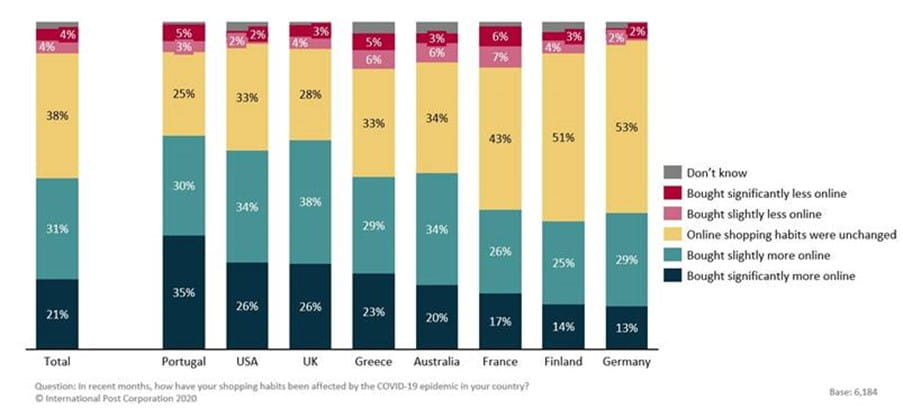
\includegraphics[scale=0.5]{images/IPC_velemeny_kutatas.jpg}
\caption{Kovid allati vásárlási szokásokról közvélemény kutatás.}
\label{fig:velemeny_kutatas}
\end{figure}

\section{Dropshipping}

\cite{21} A dropshipping az online áruházak egy olyan formája amelynél ha a vásárló rendel valamit az adott oldalról akkor nem a cég saját raktárából kapja meg a terméket. Hanem ez a cég csak egy harmadik féltől egy nagykereskedőtől vásárolja meg a terméket és azt közvetítti a vásárlónak. Így csak az értékesítést és a szállítást intézi az adott cég. 

\begin{figure}[h]
\centering
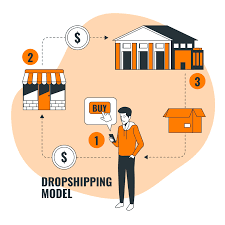
\includegraphics[scale=1.3]{images/dropshipping.png}
\caption{A dropshipping bemutatója \cite{22}}
\label{fig:dropshipping_modell}
\end{figure}

\subsection{Dropshipping előnyei}

\begin{itemize}
    \item \textbf{Kevesebb tőkét igényel és egyszerűbb beindítani}
    
Ez az egyik legnagyobb előnye mivel nincs szükség kezdő tőkére, hogy az ember egy ilyen webáruházat beindítson. Ez az miatt lehet, mert nem kell egy állandó árukészletet fen tartania egy raktár épületben, csak amikor rendelést kap, azt egy harmadik féltől kell megrendelnie. E miatt az értékesítő megspórolja a raktárépület bérlését, a csomagolási és szállítási költségeket, a készlet nyomon követését és fenntartását.

    \item \textbf{Alacsony fix költségek}
    
A fix készlet hiánya miatt sokat spórol a fenntartó, de nem csak ez az egyik fő indok, ami miatt olcsó. Nincs szüksége alkalmazottak felvevésére és telephely fenntartására ehhez a webáruház üzemeltetéseshez elég egy számítógép vagy laptop ritkábbik esetekben csak egy mobil telefon. E miatt a havi költségek igen minimálisak persze ez az összeg is növekedni fog ha az üzlet növekszik és ilyenkor már egy egyszerű mobiltelefon nem lesz elegendő. De továbbra is egy jóval olcsóbb megoldás mint más típusú webáruház üzemeltetése.

    \item \textbf{Rugalmas munkavégzési hely}
    
Ha az üzemeltető egy biztonságos és gyors internetkapcsolattal felszerelt helyen van akár onnan is dolgozhat. Egyetlen lényeg van, hogy tudjon kommunikálni a megrendelővel és a nagykereskedésekkel.

    \item \textbf{Óriási kínálat}
    
Mivel nem kell az árucikket előre megvásárolni így az üzletben óriási készletett kínálhat a vevőknek. ha egy nagykereskedő kínál egy terméket, azt a dropshipping üzlet is feltüntetheti minden extra költség nélkül.

    \item \textbf{Könnyedén skálázható}
    
Ha egy üzlethez az átlagosnál több megrendelés érkezik, azzal, jóval több munka van. De a dropshipping nagy előnye hogy a megrendelések nagy részét a nagykereskedések intézik.

\end{itemize}

\subsection{Dropshipping hátrányai}

\begin{itemize}
    \item Minimális profit
    
Ez a legnagyobb hátránya mivel könnyű belekezdeni, rengetegen bele is kezdenek így hatalmas a versenygés. Némely kereskedő a nagyon alacsony árakkal akarja magához vonzani a vevőket. Ez okból viszont nagyon alacsony lesz a profitjuk is, de ez az alacsony költségek miatt nem akkor probléma számukra. Mivel a vásárlókat csak az áru ára érdekli így még a kereskedőnek lehet jó profitja, ha sokan vásárolnak ott. Viszont a piac telítettsége miatt egyre kevésbé éri meg a dropshippinggel foglalkozni mivel annyira alacsony haszon folyik be belőle.

    \item Készletproblémák
    
Amikor egy hagyományos kereskedő a saját raktárkészletét kezeli, könnyedén nyomon követheti, hogy mennyi termék áll rendelkezésére. Viszont, ha valaki dropshipping kereskedőként a nagykereskedők raktárkészleteire támaszkodik, fennáll a veszélye annak, hogy a készletek gyorsan elfogynak. Ebben az esetben ugyanis minden más dropshipping kereskedő is ugyanezen készletekre hagyatkozik, ráadásul a hagyományos viszonteladóknak is időnként fel kell tölteniük saját készleteiket.

    \item Szállítási nehézségek
    
Általában egy dropshipping kereskedő több nagykereskedéssel dolgozik egyszerre így sokkal nehezebb nyomon követni a szállítási költségeket.

Például ha több terméket rendel és mindegyik terméket más nagykereskedőtől, akkor ott több szállítási költséget kell fizetni. Ezt a plusz összeget viszont nem szabad ráterhelni a vevőre mert úgy fogja érezni hogy túlvan árazva a szállítás.

\end{itemize}


\chapter{4.Fejlesztés}

A technológiák kiválasztása után, de még a web áruház lefejlesztése előtt a következő lépés az oldal kinézetének megtervezés. A web áruházamat úgy képzeltem el, amely képes nagy mennyiségű termék megjelenítésére és képes e termékek tárolására adatbázisban.  Az oldal megtervezésénél oda kell figyelni, hogy fel legyen szerelve egy egyszerűbb keresővel és szűrési lehetőségekkel, hogy a jövőbeli felhasználók számára könnyen kezelhető legyen. Olyan oldalt akartam volna létrehozni, amelyet a jövőbeli felhasználók előszeretettel fognak használni a későbbiekben.

\section{Oldalak megtervezése}

Két féle típusú oldalt terveztem meg. Az első azok az oldalaknak a csoportja, amelyeket azok a felhasználók láthatnak, amelyek még nem jelentkeztek be az oldalra. Ebbe a csoportba soroltam be azokat az oldalakat, amely fogadja a felhasználót az oldal meglátogatásakor, továbbá a bejelentkező, regisztrációs oldal, termékek általános megtekintését és a kosár ahol megnézheti a felhasználó a vásárolni kívánt termékeket. A második csoport azokat az oldalakat tartalmazza, amelyeket a felhasználók és a regisztráció és a bejelentkezés után láthatnak, ilyen oldalak a pénztár és a fizetés, amelyeket csak a bejelentkezés után tekinthet meg a felhasználó.

Az egyszerűbb kezelhetőségek miatt az oldalt komponensekre osztottam fel azon belül is oldalakra (pages) és részlegekre (partials). A részlegekre azért volt szükség, mert némely oldalakat több komponensből állítottam össze. Ezekre a kód egyszerűsítése miatt volt szükség vagy, éppen azért mert némely részleget több oldalon is felhasználtam.\\

A komponensek ez alapján:\\

\textbf{Pages}
\begin{itemize}
    \item Cart – ez a kosár ez tartalmazza azokat a termékeket, amelyeket a vásárló meg szeretne venni.
    \item Checkout – Ezen az oldalon tekintheti meg a felhasználó a megvásárolni kívánt termékek és áruk összesítését. További itt található a megrendelési űrlap és egy térkép a szállítás helyének kiválasztásához.
    \item Coin – ezen az oldalon láthatják nagyban a termékeket
    \item Home – ez az alap oldal ahol az összes termék fel van sorolva
    \item Login – ez a bejelentkezési oldal
    \item Payment – ez hasonló a checkout-hoz de ez után már a fizetés jön
    \item Register –ez a regisztrációs oldal
\end{itemize}

\textbf{Partials}
\begin{itemize}
    \item default-button – az alap gombok komponense
    \item header – az oldalak fejléce
    \item input-container – a login register és a checkout komponenseknél a beviteli mezők összegzésehez
    \item input-validation – a beviteli mezők ellenőrzéséhez használtam
    \item loading – töltő képernyő
    \item map – térkép a checkout-hoz
    \item not-found – gomb a főoldalra való visszatéréshez
    \item order-items-list – rendelt termékek listája
    \item search - kereséshez
    \item star-rating – a termék ritkaságának a jelöléséhez
    \item tags – szűréshez
    \item text-input – beviteli mezők
    \item title – címek
\end{itemize}

\section{Oldalak leírása}
A home oldal megtervezésénél és elkészítésénél egy olyan oldalt akartam létrehozni, amelyre a jövőbeli felhasználók szívesen visszatérnek. Ezt próbáltam megoldani egy minimalista stílussal. Az oldal látható a kereső, amelyben kereshetünk az adott termékek után. Ez alatt a különféle termékekre szűrhetünk különböző címkék alapján attól függően, hogy az adott termékeknek milyen tulajdonságaik vannak. Továbbá a címkék alatt kis kártyák láthatóak ahol a termékek láthatóak. Minden kis kártyán, helyett kapott a termékről egy kép, a termék neve és mellette egy szívecske, amely azt jelzi, hogy az adott terméket mennyire kedvence a vásárlóknak. Továbbá a kártya tartalmazz egy csillag rendszert, amely azt mutatja, hogy a termék mennyire ritka. Ez alatt foglal helyet a termék tulajdonságai és ára forintban megadva.

\begin{figure}[h]
\centering
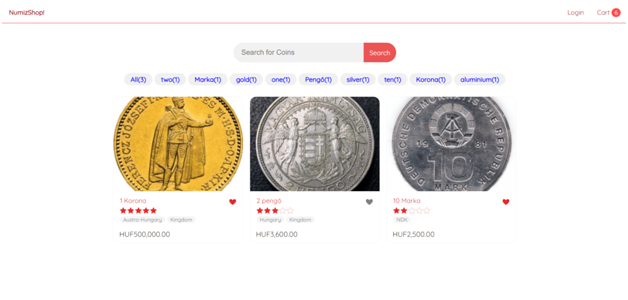
\includegraphics[scale=1]{images/home.png}
\caption{A főoldal megjelenítése.}
\label{fig:fo_oldal}
\end{figure}

Minden oldal tetején látható a fejléc sáv. Az oldal logójára kattintva mindig a fő oldalra fog vezényelni. A jobb felső sarokban a login gombra kattintva a bejelentkező oldalra vezérel át ahol képesek vagyunk belépni vagy ha még nincs felhasználói fiókunk onnan tudunk átnavigálni a regisztrációs oldalra. A login gomb mellett található a cart gomb, amely tovább navigál a kosárhoz. Ezen a gombon folyamatosan láthatjuk, hogy mennyi terméket helyeztünk a kosárba. Ez a kis funkciót azért raktam bele az oldalba, hogy a vásárlóknak még kényelmesebb legyen az oldal használat így nincs szükségük belépni a kosárba, hogy tudják, hogy mennyi termékük van már. A login oldal egyszerűen van felépítve csak középen a belépő űrlap és alatta egy gomb, ha a regisztrációs oldalra akar átnavigálni az ember. A register oldal is így van, felépítve csak itt regisztrációs űrlap van és a gomb a login oldalra vezényel át. A coin oldal akkor jelenik, meg amikor a fő oldalon rákattintunk valamelyik termék kártyájára. Ez további információkat tartalmaz a termékről, mint például a pontos névértéke, az anyaga és a pontos neve. Ezen felül nagyobb méretben láthatjuk az adott terméket.

A cart oldalra átnavigálva láthatjuk a kosarunk tartalmát. Itt a megvásárolni kívánt termékek felvannak sorolva egymás alatt kis léceken. Ezeken a léceken állíthatjuk hogy az adott termékből mennyit szeretnénk vásárolni és hogy nagyobb mennyiségben mennyibe fog kerülni. Viszont arra az esetre is gondolni kell ha a vásárló csak félre kattintott így egy törlés gombot is elhelyeztem amivel az adott terméket eltávolíthatjuk a kosárból. A lécek mellett egy összeítő fült hoztam létre amely tartalmazza a termékek össz árát és ártéket ez alatt pedig egy gomb amely a pénztárhoz vezet tovább. Viszont a pénztárhoz csak bejelentkezés után lehet navigálni. Ezért ha regisztráció nélkül nyomunk a gombra akkor a bejelentkezési oldalra fog navigálni.

\begin{figure}[h]
\centering
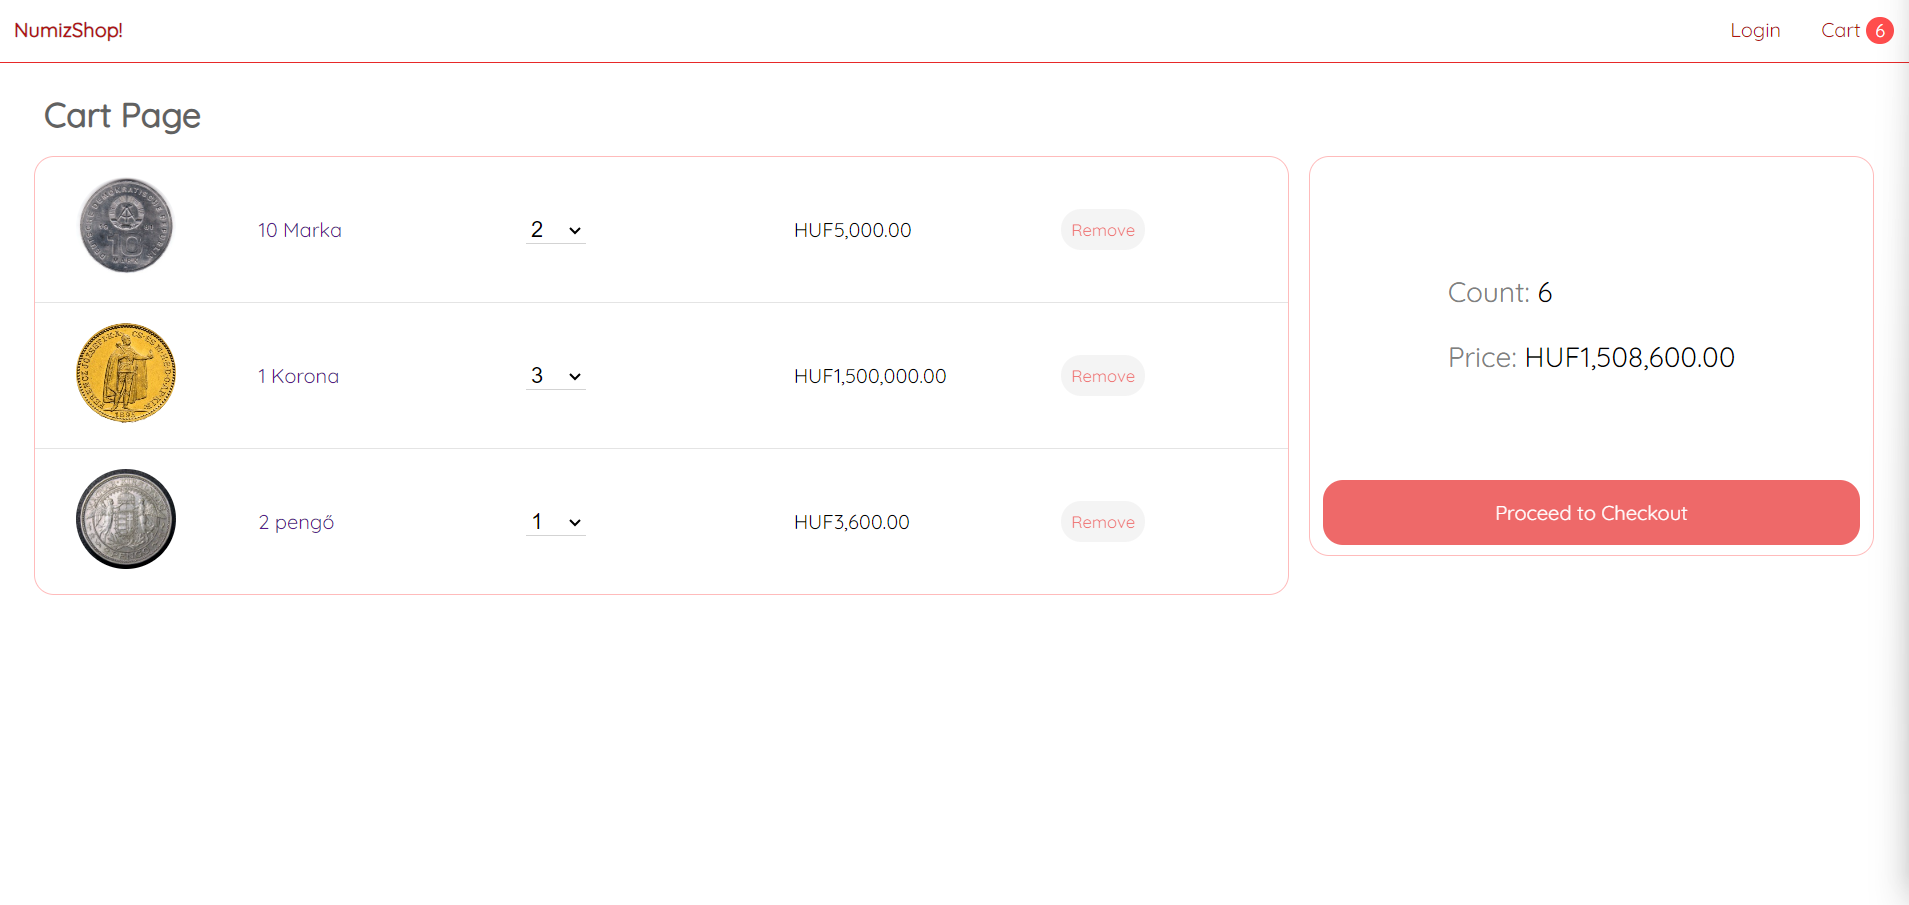
\includegraphics[scale=0.3]{images/cart.png}
\caption{A kosár megjelenítése a webáruházban.}
\label{fig:kosar}
\end{figure}

Ha már viszont be vagyunk jelentkezve és tovább navigálunk a pénztár oldalra. Akkor itt is láthatjuk a megvásárolni kívánt termékeket azok össz és darab értékét, és hogy melyik termékből mennyit akarunk vásárolni hasonlóan a kosár oldalához. Továbbá meg kell adnunk a vevő nevét és lakcímét. Ezek mellett található egy világtérkép, amivel a pontos helyzetünket adhatjuk meg a szállítás megkönnyítéséhez. A térképen található egy gomb, amellyel rögtön a saját helyzetünkhöz ugrik a térkép ezzel a felhasználó dolgát megkönnyítve a kellemesebb használat érdekében. A térkép létrehozásához egy külön komponenst azon belül is egy részleget hoztam létre ezt annak az érdekében, hogy a kód átláthatóbb legyen mivel több beállítást is véghez kellett vinni a térképen.

\begin{figure}[h]
\centering
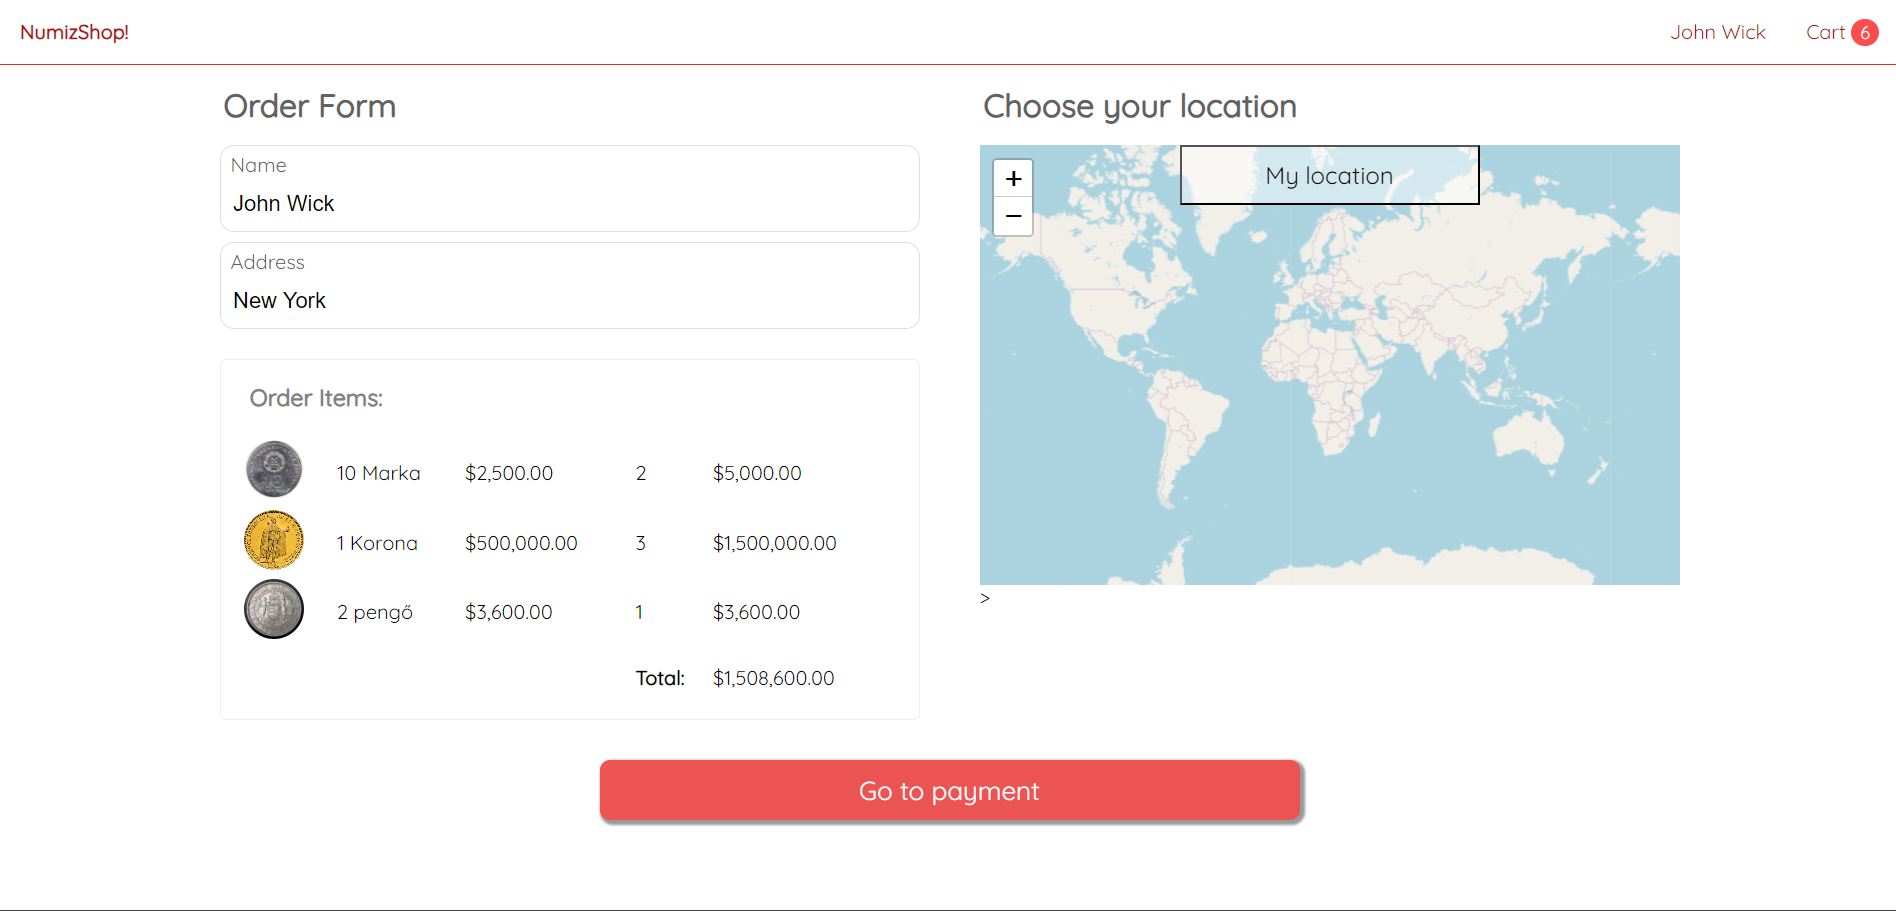
\includegraphics[scale=0.3]{images/checkout.png}
\caption{A pénztár megjelenítése a webáruházban.}
\label{fig:penztar}
\end{figure}

Ha a pénztár oldal alján tovább navigálunk payment (fizetés) oldalra ugyan az az oldal fog fogadni, mint a pénztár oldalán viszont itt már az oldal alján egy paypal vagy más egyébb fizetési mód fogadja a felhasználót ez a része viszont nincs lefejlesztve, de erre a jövőbeli terveknél majd visszatérek. Azokban a pillanatokban, amikor két oldal között navigálunk, és az oldal tölt arra az esetre létrehoztam egy komponenst, amely a töltőképernyőt biztosítja ez a partials mappában a loading az itt található töltő képet a loading.io [hivatkozás] oldal segítségével hoztam létre saját magam. A jövőbeli felhasználók segítségére létrehoztam még egy fontos komponenst a partials mappába az input-validation-t.

\begin{figure}[h]
\centering
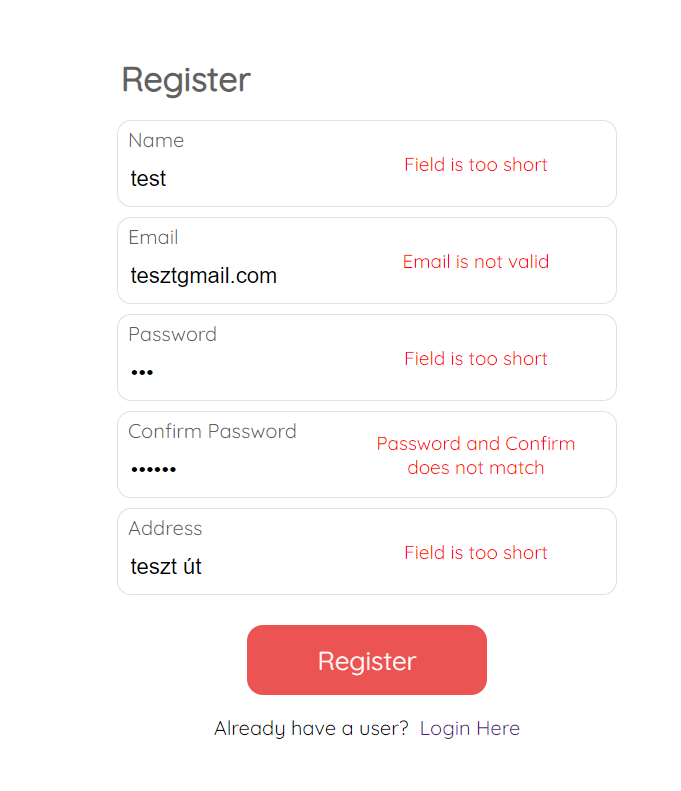
\includegraphics[scale=0.6]{images/validation.png}
\caption{A beviteli mezők validálása.}
\label{fig:validacio}
\end{figure}

Ezt akkor használom, amikor regisztrálnánk vagy bejelentkeznénk. Ez a komponens ellenőrzi azt, hogy a beviteli mezőkben érvényes adatokat adjanak meg a felhasználók. Regisztrációnál szól, ha túl rövid nevet vagy jelszót ad meg a felhasználó vagy például nem megfelelő formátumú az email cím. Ez a komponens is azért hoztam létre ami az egyik fő célom is volt hogy egy olyan webáruházat hozzak létre amelyet a felhasználók könnyedén kezelni tudnak és baráti a kezelő felülete ami arra sarkalja őket hogy vissza térjenek később is ide.

\subsection{Adatbázis}
Miután már nagyjából összeállt a fejemben hogy hogyan is szeretném, hogy kinézzen a webáruházam frontend része. A következő rész az adatbázis megtervezése volt. Ennek a résznek a megtervezése az egyik legfontosabb feladat, mert ennek függvényében változhat a későbbiekben a frontend kinézete. Meg a program írása közben már pontosan tudtam, hogy milyen adatokkal is kell dolgoznom. Adatbázisnak az áruházhoz a MongoDB-t választottam ezen belül is a MongoDB Atlast. Két verziója van a MongoDB-nek az egy a Compass amely egy letölthető verzió a másik az Atlas amely pedig felhő alapú. Én azért az Atlas mellett döntöttem, mert számomra egyszerűbben használható volt.

Amikor terveztem a frontendet hat darab modell-t hoztam létre ezekből. Ezek közül háromra van biztosan szükségünk meg egyre még szükségünk lehet ha szűrni akarunk az adatbázisban. A három fő modell a Coins, a User és az Order. A szűrő modell pedig a Tag.\\

Ezek a modellek a következő attribútumokat tartalmazzák:

Coins:
\begin{itemize}
    \item id – az érme egyedi azonosítója
    \item name – az érme neve
    \item price – az érme ára
    \item tags – az érme tulajdonságai
    \item favorite – ez mutatja, hogy az érme a kedvencek között van -e
    \item stars – ez mutatja az adott érme ritkaságát
    \item imageUrl – az érméről kép
    \item origins – az érme eredete
\end{itemize}

User:
\begin{itemize}
    \item id – a felhasználó egyedi azonosítója
    \item email – a felhasználó saját email címét tartalmazza, egy email címet csak egyszer lehet használni mivel az oldalra való belépés során a felhasználónak az email címét és jelszavát kell megadnia
    \item name – a felhasználó neve 5 karakternél hosszabbnak kell lenni a regisztrációs validációk miatt
    \item address – a felhasználó címét tartalmazza
    \item token - a felhasználóhoz tartozó tokent tartalmazza
    \item isAdmin – azt tartalmazza, hogy az adott felhasználó az oldalon milyen pozíciót tölt be
\end{itemize}

Order:
\begin{itemize}
    \item id – az érméknek egyedi azonosítója van, amelyeket a cart modell-be helyezünk
    \item items – ez tartalmazza a termék árát és darab számát 
    \item totalPrice – ez tartalmazza a kosár tartalmának teljes összegét
    \item name – ez tartalmazza a vásárló nevét
    \item address – ez tartalmazza a vásárló címét
    \item addressLatLng – ez tartalmazza a vásárló címét, amelyet a térképpel adott meg
    \item paymentId – ez tartalmazza a fizetés egyedi azonosítóját
    \item createdAt – ez tartalmazza, hogy mikor keletkezet a rendelés
    \item status – ez tartalmazza a rendelés állapotát
\end{itemize}

Ezek mellett a kisebb modellek igazából csak a nagyobb modellek kiszolgálására hoztam létre ilyen modell a CartItem amely az Order modell items attribútumát adja. Mint már fentebb említettem a szűrésekhez a Tag modellt használom, melynek csak két attribútuma van a name és a count ennek segítségével tudok az érmék között szűrést végre hajtani.

\subsection{Alap adatok feltöltése}
Az oldal teszteléséhez szükségem volt alap adatokra, ezért a coun.router.ts-be és a user.router.ts-be létrehoztam egy-egy útvűlasztó(router) endpointot amely a /seed útvonalon elérhető. Ezek a végpontok (endpoint) egy aszinkron funkciót hajtanak végre, amely, amelyek az adatbázisba adatokat helyeznek el, ezt angolul seed-nek nevezzük. Az adatokat csak abban az esetben helyezi el az adatbázisban, hogy ha még nincsenek az adatbázisban. A kód pontos működése: a router.get ”/seed” útvonalra érkező GET kéréseket kezel. Ehhez segítséget nyújt az asyncHandler függvény amely megkönnyíti az aszinkron kódblokkok kezelését. Az async (req, res) => aszinkron funkció végrehajtódik amikor a útvonalon való kérés megtörténik a req tartalmazza az érkező kérés adatait, a res-sel pedig választ küldhetünk vissza a kliensnek. Ez után megszámolja az adatbázisban tárolt CoinModel dokumentumainak számát aszinkron módon. Ehhez az ”await”-et használtam, hogy a végrehajtás megálljon, amíg a számlálás folyik. A számolás után ellenőrzöm hogy van-e már adat az adatbázisban. Abban az esetben, ha már van, küld egy választ a kliensnek a ”Seed is already done!” Üzenettel majd a funkció befejeződik. Ha viszont még nincs adat az adatbázisban, akkor a CoinModell alapján létrehoz egy vagy több dokumentumot az adatbázisban. Ezeket az adatokat a ’sample\_coins’ tömbből veszi, majd minden elemhez egy ’id’ tulajdonságot hozzáad, melynek értéke: null. Az ”await”-et ismét használva várakozni fog még az adatbázisba való feltöltés befejeződik. Majd a res.send segítségével választ küld a kliensnek hogy ”Seed is done” tehát a feltöltés (seedelés) folyamat sikeresen megtörtént.

\begin{python}[caption={Alap adatok feltöltése},captionpos=b]
  router.get("/seed", asyncHandler(
  async (req, res) => {
     const usersCount = await UserModel.countDocuments();
     if(usersCount> 0){
       res.send("Seed is already done!");
       return;
     }
 
     await UserModel.create(sample_users);
     res.send("Seed Is Done!");
 }
 ))
\end{python}

\section{Azonosítás megoldása}
Miután megterveztem az adatbázist és a weboldal frontend részét a következő lépés maga a webáruház létrehozása. Mivel egy ilyen jellegű weboldalt remélhetőleg nagy mennyiségű felhasználó fogja látogatni és vásárlásra használni. Ezért fontos szempont volt az elkészítés során a biztonság. Hogy biztosítsam a felhasználók adatait. Szerencsére erre több módszer is létezik. A következőkben az általam használt módokat fogom bemutatni.

Mivel az oldalon való vásárláshoz, regisztrációhoz van szükség ezért a regisztráció és bejelentkező részt írtam meg először. Ugyan is itt van a legnagyobb szükség a biztonságra. A regisztráció folyamán miután a frontend megkapta az adatokat először validálni fogja azt, hogy megfelelnek a megadott jellemzőknek ilyen például, hogy öt karakternél hosszabb név kell, tíz karakternél hosszabb cím, vagy ami segít a felhasználónak, hogy biztosan jó jelszót adjon, meg hogy egyszer ismételten meg kell adnia a jövőbeli jelszavát. Abban az esetben, ha van azonos email cím akkor az oldal szólni fog hogy már regisztrált. Ezek mellet ellenőrzi, hogy a megadott email cím létezik-e már mivel egy email címet csak egyszer lehet használni mivel az oldalra való belépés során a felhasználónak az email címét és jelszavát kell megadnia. Amennyiben sikeres a regisztráció a jelszót hash-elni fogja és tovább küldi az adatbázisnak. 

\subsection{Jelszó titkosítás}
A jelszó védelmére az egyik legalapvetőbb módszer a hashelés ezért választottam én is ezt a módszert. Viszont hozzá kell tenni, hogy ez nem a legbiztonságosabb módszer mivel, vannak olyanok, akik ennek gyengeségeit már ki tudják használni. A működési elve a következő: Kap egy betűkből és számokból álló kombinációt, ezt az algoritmus átalakítja hexadecimális formába bár ez a hash algoritmustól is függ. Előnye hogy bármilyen hosszúságú lehet a jelszó (betűk és számok kombinációja)

\newpage

\begin{python}[caption={Regisztráció},captionpos=b]
  router.post('/register', asyncHandler(
  async (req, res) => {
    const {name, email, password, address} = req.body;
    const user = await UserModel.findOne({email});
    if(user){
      res.status(HTTP_BAD_REQUEST)
      .send('User is already exist, please login!');
      return;
    }

    const encryptedPassword = await bcrypt.hash(password, 10);

    const newUser:User = {
      id:'',
      name,
      email: email.toLowerCase(),
      password: encryptedPassword,
      address,
      isAdmin: false
    }

    const dbUser = await UserModel.create(newUser);
    res.send(generateTokenReponse(dbUser));
  }
))
\end{python}

A bejelentkezés során a jelszót szintúgy hash-elem és így hasonlítom össze a már adatbázisban lévővel. Fentebb már említettem, hogy a hash nem a legbiztonságosabb fajta módszer ezért bcrypt hashelést használtam. Amely saltingot használ az úgy nevezet rainbow table támadások ellen. Mivel a hash hossza mindig azonos és a hashelni kívánt karakter sorozat hossza is minden esetben azonos ezt használja ki a rainbow table támadás is. A jelszavak védelmére ezért kitalálták a saltingot. Itt a jelszó mellé random adatokat rak a bcrypt ezzel védelmet nyújtva a támadások ellen.

\newpage

\begin{python}[caption={Bejelentkezés},captionpos=b]
  router.post("/login", asyncHandler(
  async (req, res) => {
    const {email, password} = req.body;
    const user = await UserModel.findOne({email});
  
     if(user && (await bcrypt.compare(password,user.password))) {
      res.send(generateTokenReponse(user));
     }
     else{
       res.status(HTTP_BAD_REQUEST)
       .send("Username or password is invalid!");
     }
  
  }
))
\end{python}

\subsection{Web Token és Interceptor}
Az adatok biztonsága még így se garantált ezért a sikeres bejelentkezés során generáltatok egy JSON web tokent. Viszont a JSON web token generálása során oda kell figyelni, hogy fontosabb adatokat nem szabad beletenni, mint például bankkártya adatokat vagy hasonló dolgokat.
A generálását én adtam meg az adatok segítségével az alábbi négy részt generálom bele.

\begin{itemize}
    \item User ID -  ezzel lehet azonosítani a, belépet felhasználót
    \item User email – a felhasználó email címe
    \item User isAdmin ebből tudjuk, meg hogy az adott felhasználó milyen pozíciót tölt be az oldalon
    \item JWT\_SECRET ez lesz a titkos kód
\end{itemize}

Az én esetemben ebből a négy dologból fog létrejönni a token. Sikeres bejelentkezés esetén a szerver visszaküldi a tokent és ezt local storage-ban fogja tárolni. Viszont ez így még nem teljesen biztonságos ezért http Interceptort kell használnunk, amely a HTTP request és handler használatával fogja kezelni a beérkező kéréseket. Erre azért van szükség a local storage-t a fejlesztői eszközökkel adatot vihetünk a local storage-ba és már benne lévőket akár felül is írhatjuk.

Az interceptor működése az alábbi: Sikeres bejelentkezés után a már feltöltött tokent lekérdezi abban az esetben, ha a local storage tartalmazza azt akkor leklónozza és a headerben token-ként tárolni fogja azt. Ez után a headerből leklónozott tokent és a szerveren tárolt JWT\_SECRET titkos kódunkat összehasonlítja.

\begin{python}[caption={Interceptor},captionpos=b]
    intercept(request: HttpRequest<unknown>,
    next: HttpHandler): Observable<HttpEvent<unknown>> {
    const user = this.userService.currentUser;
    if(user.token)
    {
      request = request.clone({
        setHeaders:{
          access_token: user.token
        }
      })
    }
    return next.handle(request);
  }
\end{python}

\subsection{Middleware Authorization}
Mivel a főbb funkciókat az oldalon csak akkor lehet használni, ha a felhasználó be van jelentkezve és ezekhez a műveletekhez a oldalnak szüksége van az adott felhasználó id-ra. Ez okból az eddigi védelmek még nem voltak elegendőek még foglalkoznunk kell azokkal a felhasználókkal is, akik úgy próbálják elérni az oldal korlátozott részeit, hogy nem lépnek be. Ez pont azért fontos, mert ha úgy lépne be valaki az oldal e részeire, hogy nincs felhasználói id-je akkor számára ezek a funkciók nem fognak működni. Ezen probléma megoldásásra middleware authorizationt használok. Ez egy olyan szűrő, amely kérések feldolgozása előtt vagy után ellenőrzi, hogy a felhasználó jogosult-e az adott művelet végrehajtására. Ez a szűrő általában az alkalmazás biztonsági rétegét erősíti meg, és megkönnyíti a fejlesztők számára az engedélyek és az autentikáció kezelését. Jelen esetben feladata a fejlécből lekérdezi a token majd ellenőrzi, hogy a token létezik-e, és ha nem a választ elküldi a HTTP\_UNAUTHORIZED státusszal tehát nem rendelkezik a megfelelő jogosultságokkal. A JSON web token-t ellenőrzi a verify függvénnyel amennyiben sikeres hozzá a req.user változóhoz. Azonban ha a JSON Web Token ellenőrzése sikertelen (például lejárt vagy érvénytelen) akkor szintén http\_UNAUTHORIZED státuszt küld vissza. Csak ez után hívja meg a middleware a next függvény, hogy továbbítsa a vezérlést a végpontoknak.

\begin{python}[caption={Middleware Authorization},captionpos=b]
import { verify } from "jsonwebtoken";
import { HTTP_UNAUTHORIZED } from "../constants/http_status";

export default (req: any, res: any, next: any) => {
    const token = req.headers.access_token as string;
    if(!token) return res.status(HTTP_UNAUTHORIZED).send();

    try{
        const decodedUser = verify(token, process.env.JWT_SECRET!);
        req.user = decodedUser;
    }catch(error){
        res.status(HTTP_UNAUTHORIZED).send();
    }

    return next();
}
\end{python}

\section{A termék megvétele}
Mielőtt még bejelentkeztünk, de persze utána is lehetőségünk van terméket helyezni a bevásárló kosárban. A fő oldalon a kiválasztott éremre kattintva átvisz a termék külön oldalára ahol a leírásuk is található ezen az oldalon az „Add to Cart” gombra rákattintva az adott termék bele kerül a kosarunkba. Minden gomb a dinamikus tömbnek köszönhetően megkapja az adott termék azonosítóját. Amikor a kosárba helyezzük a local storage-ba kerül az azonosító. Amikor átlépünk, a kosárba meghívódik egy metódus, amely kilistázza az eddigi termékeket és összehasonlítja az azonosítójukat amennyiben megegyezik, abban az esetben megjelenik a frontenden a kosárban. Megvásárlás esetén az érmék adatait feltölti az Order modellbe majd hozzá adja a felhasználó nevét, címét, a pontos címét és a dátumot. Azonban amikor visszalépünk a rendelés törlődik a local storage-ból.

A pontos működése a következő: Először is egy middleware-t használok, amely azonosítja és ellenőrzi a felhasználó hitelességét. Hogy biztosan csak olyan felhasználó tudjon vásárolni amelyik, be van jelentkezve. Ez után az útvonal egy POST kérést fogad a /create végponton keresztül. Az aszinkron műveleteket az asyncHandler segítségével kezelem. Majd ellenőrzi, hogy ellenőrzi, hogy a request body-ban lévő rendelés tartalmaz-e legalább egy tételt. Abban az esetben, ha a kosár üres HTTP\_BAD\_REQUEST státuszkódot add vissza válaszként és egy ”Cart is empty” üzenetet küld vissza. Ezt követően ellenőrzi, hogy van-e olyan rendelés, amelynek státusza ”NEW” és ugyanazon felhasználóhoz tartozik, majd létrehoz egy új rendelést és ment azt az adatbázisba és válaszként visszaküldi az új rendelést. 

\begin{python}[caption={Rendelés létrehozása},captionpos=b]
router.post('/create',
asyncHandler(async (req:any, res:any) => {
    const requestOrder = req.body;

    if(requestOrder.items.length <= 0){
        res.status(HTTP_BAD_REQUEST).send('Cart is empty');
        return;
    }

    await OrderModel.deleteOne({
        user: req.user.id,
        status: OrderStatus.NEW
    })

    const newOrder = new OrderModel({...requestOrder,user: req.user.id})
    await newOrder.save();
    res.send(newOrder);

}))
\end{python}

Következő útvonal a /newOrderForCurrentUser. Itt az útvonal GET kéréseket fogad el ettől a végponttól majd úgyszintén az aszinkron műveleteket az asyncHandler segítségével kezeli. Lekérdezi azokat a rendeléseket az adatbázisból, amelynek státusza ”NEW” és a felhasználó azonosítója megegyezik a bejelentkezett felhasználóval. Ha talál, ilyen rendelést válaszként visszaküldi azt, egyébként pedig HTTP\_BAD\_REQUEST státuszkóddal válaszol.

\subsection{Keresés és címkék}
Mivel a weboldalon több termék is megjelenik ezért, hogy a felhasználó könnyebben megtalálja a keresett terméket létrehoztam egy keresés komponenst. A keresést egy egészen egyszerű módon oldottam meg. Létrehoztam egy változót, amelyet a komponens arra használ, hogy ebben tárolja a keresési kifejezést. A konstruktorba injektáltam az ActivatedRoute és Router-t majd a route paraméterek változásait az activatedRoute.params.subscribe figyeli. Abban az esetben, ha változás történik és van ilyen paraméter, akkor azt a már fentebb említett változóba elmenti. Ez után egy külön függvény amelyet ’search’-nek neveztem el, keresést indít a Router segítségével. Ha van érvényes keresési kifejezés, akkor a felhasználót átirányítja a megadott keresési kifejezéssel ellátott útvonalra. 

\begin{python}[caption={Keresés},captionpos=b]
  searchTerm = '';

  constructor(activatedRoute:ActivatedRoute, private router:Router) {
    activatedRoute.params.subscribe((params) => {
      if(params.searchTerm) this.searchTerm = params.searchTerm;
    });
  }

  ngOnInit(): void {
  }

  search(term:string):void{
    if(term)
    this.router.navigateByUrl('/search/' + term);
  }
\end{python}

A termékek keresésére nem csak ezt az egyszerű kereső komponenst hoztam létre, hanem a fő oldalon a kereső mező alatt címkéket (tag) hoztam létre. A szűrési típusok közül azért erre döntöttem mivel az oldal csak régi pénz érmékkel foglalkozik és nincs különösen túl sok tulajdonságuk így nem éreztem szükségét egy nagyobb bonyolultabb szűrési módszernek. Ennek a működése a következő. A címkéket a komponens egy tags nevű változóban tárolja. A konstruktorba injektáltam a CoinServicet majd meghívódik a coinService getAllTags() metódusa. Ez a metódus egy HTTP GET kérést indít a COIN\_TAGS\_URL végpontra, amely válaszként egy tömböt vár amelyben a már megadott típusú ’tag’ elemeket tartalmazza. Ezt az eredményt ’Observable’-ként adja vissza. Az Observable egy olyan objektum, amely egy vagy több érték érkezését várja, majd értesítést küld azoknak a részeknek az alkalmazásban, amelyek fel vannak iratkozva rá. Azért így csináltam, meg mivel amikor az alkalmazás megjeleníti egy falhasználó számára a választható opcióként. Akkor ezek a címkék dinamikusan kerülnek betöltésre a szerverről. Ezután a feliratkozott komponensek lefrissülnek, amikor a címkék megváltoznak. Ez miatt képes az alkalmazás dinamikusan kezelni a címkék frissítését a szerverről.

\section{Térkép hozzáadása}
Egy webáruháznál térkép használata a kiszállítási címhez számos előnnyel járhat mind az ügyfelek, mind a vállalkozás számára. Ennek több indoka is van: 

Először is a felhasználói élmény javítása. A térkép használatával a vásárlók könnyen és gyorsan kiválaszthatják a kiszállítási címüket. Ez például abban az esetben lehet hasznos, ha a vásárlók még nem ismerik eléggé jól a kiszállítási területet. A felhasználók pontosabban és egyértelműben megadhatják a címüket, amellyel csökkenthetik a szállítási hibák valószínűségét és az is nagy megnyugvást tud adni a vásárlóknak, hogy a térkép segítségével valós idejűleg a csomaguk aktuális tartózkodási helyét. 
Továbbá a vállalkozások is egyszerűbben tervezhetik meg a szállítási útvonalakat ezzel csökkentve az üzemenyagköltségüket. Ráadásul a térkép használata könnyen integrálható üzleti rendszerekkel és alkalmazásokkal, amely segíthet az autómatizálásban. 

Ezek az indokok miatt döntöttem én is arra, hogy szükség lesz az én webáruházamnak is egy térképre ezzel még kívánatosabbá tenni a jövőbeli vásárlóknak. Persze ezt az összes funkciót még nem tartalmazza, de a felhasználóknak már lehetőségük van kiválasztani a saját tartózkodási helyüket.

A térkép megvalósításához a leaflet JavaScript könyvtárat választottam, mivel ez egy könnyen tanulható és egyszerűen használható térképkeretrendszer. Annak köszönhetően, hogy moduláris felépítésű lehetővé tette számomra hogy csak azokat a funkciókat és modulokat használjam amelyekre ténylegesen szükségem van, ezzel csökkentve a felesleges kódrészeket melynek hála a program teljesítménye is növekedett. 

Először is létrehoztam egy location.service.ts service-t ide importáltam a ’LatLngLiteralt’-t a leaflet könyvtárból és az ’Observable’-t az ’rxjs’ könytárból. Majd létrehoztam a ’getCurrentLocation’ metódust amely egy LatLngLiteral típusú observable-t add vissza. Ez ellenőrzi, hogy a Geolocation API elérhető-e a böngészőben. Abban az esetben, ha elérhető meghívja a navigator.geolocation.getCurrentPositon függvényt, hogy lekérdezhesse az aktuális pozíciót. Ez után két lehetőség van, siker esetén kibocsájtja a szálességi és hosszúsági koordinátákat, hiba esetén pedig az observer.error segítségével a hibát bocsájtja ki.

\begin{python}[caption={Aktuális lokáció megadása},captionpos=b]
    getCurrentLocation(): Observable<LatLngLiteral>{
    return new Observable((observer) => {
      if(!navigator.geolocation) return;

      return navigator.geolocation.getCurrentPosition(
        (pos) => {
          observer.next({
            lat: pos.coords.latitude,
            lng: pos.coords.longitude
          })
        },
        (error) => {
          observer.error(error);
        }
      )
    })
  }
\end{python}

A service után létrehoztam a map komponenst amelybe inmplementáltam az OnChange interfészt, hogy a komponens érzékeljen mindent változást az @Input változóinak megváltozásairól. Két fontos változót hoztam létre, az ’order’-t @Input dekorátorral ellátva amely ’Order típusú objektumot tartalmaz, és a ’readonly’ változót szintén @Input dekorátorral ellátva, amely azt határroza meg hogy a térkép csak olvasható módban van-e. Létrehoztam öt darab metódust a térkép kezelésére:
\begin{itemize}
    \item showLocationOnReadonlyMode: Ez a metódus arra az esetre kell amikor csak olvasható módban van a térkép, ilyenkor a térkép mozgatását, nagyítását és egyébb interakcióit tiltja le.
    \item initializeMap: ez inicializálja a térképet
    \item findMyLocation: ez a metódus keresi meg a felhasználó aktuális tartózkodási helyét és ennek megfelelően állítja be a térképet
    \begin{python}[caption={Megadja felhasználó aktuális pozícióját},captionpos=b]
    findMyLocation(){
    this.locationService.getCurrentLocation().subscribe({
      next: (latlng) => {
        this.map.setView(latlng, this.MARKER_ZOOM_LEVEL)
        this.setMarker(latlng)
      }
    })
  }
    \end{python}
    \item setMarker: ez a metódus állítja be a térképen a megfelelő koordinátákat a jelölővel és ez a metódus felelős a jelölő mozgatásáért
    \begin{python}[caption={A felhasználó lokációjára egy jelölőt rak},captionpos=b]
    setMarker(latlng:LatLngExpression){
    this.addressLatLng = latlng as LatLng;
    if(this.currentMarker){
      this.currentMarker.setLatLng(latlng);
      return;
    }

    this.currentMarker = marker(latlng, {
      draggable: true,
      icon: this.MARKER_ICON
    }).addTo(this.map);

    this.currentMarker.on('dragend', () => {
      this.addressLatLng = this.currentMarker.getLatLng();
    })
    }
    \end{python}
    \item addressLatLng: Getter és setter metódus a cím koordinátáinak beállítására és lekérdezésére
\end{itemize}

Ezekkel a metódusokkal a komponens lehetővé teszi egy interaktív térkép megjelenítését és kezelését.
\chapter{Tesztelés}

A tesztelés a weboldal készítés egyik fontos lépése. Ezért a tesztelést én is próbáltam legjobb tudásom szerint véghezvinni. Mivel egy webáruház egy igen komplex projekt ezért számtalan részre oda kellett figyelnem a tesztelés során, amik miatt a program hibába ütközhet. Egy weboldalt különböző típusú operációs eszközzel és böngészővel ellátott eszközről fogják használni. Ez okból fontos, hogy minden platformon hibátlanul működjön, legyen az mobilról vagy asztali gépről használva. Mivel a webáruházam csak a saját gépemen elérhető nincsen publikálva az internetre így a kompatibilitási tesztelést csak szűk körűen tudtam végre hajtani. Ehhez két számítógépet és több böngészőt alkalmaztam. Itt rögtön problémába is ütköztem ugyan is a saját google chromomra letöltött egyik bővítmény akadályozta a program megfelelő futását. Megfelelő tesztelés nélkül egy ilyen probléma nem derült volna ki és ez a későbbiekben a felhasználóknak problémát okozhatott volna. Következő tesztelési forma, amit véghezvittem az úgynevezett funkcionális tesztelés. Ennek lényege, hogy ellenőrizzük, hogy a weboldal/webes alkalmazás minden részegysége a megfelelő képen működik-e. Persze tesztelni ezeket az egységeket csak akkor lehet, ha azok már készen vannak. Itt ezt a tesztelést több területre lehet bontani.\cite{23}

Hivatkozások ellenőrzése
\begin{itemize}
    \item Külső linkek
    \item Belső linkek
    \item Email linkek
    \item Törött linkek
    \item Árva oldalak
\end{itemize}

Űrlapok tesztelése:
Mivel a felhasználóknak az űrlapon keresztül kell belépniük az oldalra és az oldal funkciói csak ez után lesznek képesek használni így nagyon fontos ezek ellenőrzése.

Általánosságban ezekre kell figyelni:
\begin{itemize}
    \item Hiba jelzések
    \item Hiba üzenetek
    \item Mező validáció
    \item Kötelezően kitöltendő mezők
    \item Mező maszkolás
    \item Jelszó mezők működése
    \item Captcha működése
\end{itemize}

Az űrlap kitöltésénél kifejezeten oda figyeltem mind a bejelentkezésnél, mind a regisztrációnál hogy minden mező validálva legyen. Legyen szó az email megfelelő formátumáról vagy regisztrációnál az ismételt jelszó magadásánál mindenhova került hiba esetén hiba üzenet is, amivel segítséget nyújthatunk a felhasználóknak. Figyeltem arra is, hogy amennyiben a bejelentkezés során az adatokat hibásan adná meg a belépő az oldal akkor is szóljon neki a hibáról.

Következő tesztelési forma az úgynevezett Usability tesztelés itt ellenőriztem azt, hogy a webáruházat használó felhasználóknak mennyire kényelmes és értelmezhető az oldal használata. A legfontosabb részek, amelyeket tesztelnem kellett a navigáció és a tartalom. Először is a navigáció itt arra kellett oda figyelnem, hogy a navigáció az oldalak között megfelelően működik-e és hogy az adott menüpontok érthetőek a felhasználók számára. Ebben az esetben a menüpontok nevére próbáltam a legérhetőbben megadni. A navigációkat pedig mindegyiket egyesével leteszteltem. Ezek után a tartalmat teszteltem le. Átkellett néznem, hogy tartalmilag logikusan építettem fel a webáruházat, hogy nincsenek-e helyesírási hibák, a kártyáknál és a termékek oldalán a képek minősége megfelelő nem homályos és nem pixeles. Továbbá ilyenkor néztem meg a keresés és a címkék egyértelműek és könnyedén lehet-e őket használni.

Következőleg a felhasználói felületet teszteltem angolul UI (user interface) teszt. Mivel ezen keresztül lép kapcsolatba a felhasználó az oldalunkkal így itt is különös figyelmet kellett fordítanom a tesztelésre.

Ilyenkor az alábbi pontokat vizsgáljuk:
\begin{itemize}
    \item A felhasználói felületekre vonatkozó sztenderdeknek történő megfelelés ellenőrzése
    \item A design elemek ellenőrzése: elrendezés, színek, betűtípusok, feliratok, szöveg blokkok, szöveg formázás, nyomógombok, CTA-k, ikonok, linkek
    \item A felület tesztelése különböző felbontásokon
    \item Nyelvi változatok tesztelése
    \item Különböző eszközökön (mobil, tablet, desktop) történő tesztelés
\end{itemize}

Külön oda kellett figyelnem, hogy például az oldalon egyik kép se legyen nagyobb a másiknál, a hosszabb nevek ne lógjanak túl, hanem törjenek meg a kártyáknál. Nem lenne esztétikus, ha kilógna a szöveg vagy különféle méretűek lennének a képek. 

A program készítése közben továbbá figyelmet kellett fordítanom a regisztrálás esetén az adatok helyes tárolására főként a jelszó tárolására. Mivel regisztrációnál és bejelentkezés során is az adatok titkosítva vannak ügyelnem kellett, hogy azonos formátumban legyenek lementve, hogy a későbbiekben, amikor szükség van, az összehasonlításukra az ne okozzon problémát.

\chapter{Összefoglalás és jövőbeli tervek}

\section{Összefoglalás}
Miután befejeztem a webáruház készítését és átnéztem még egyszer utoljára összességében meg vagyok vele elégedve. Mivel sikerült a kitűzött célok nagy részét elérni és sikerült egy kisebb és egyszerűbb webáruházat létrehozni. Ennek létrehozása az kihívásokat állított elem mivel eddigi éveim alatt még nem kellett egyedül dolgoznom egy ilyen komplexebb projekten. Viszont nagy segítséget nyújtott számomra hogy barátaimmal EvoCampus projekten belül dolgoztunk hasonló programon. De ott csak egy adott részen kellett dolgoznom nem pedig a frontendel és backendel is. Ez egy teljesen új tapasztalat volt, mert nagy a különbség hogy egy több fős csapattal dolgozni ahol a backendnek is csak egy szeparált részén kellett dolgoznom vagy pedig minden egyes részének a programnak nekem kellett megcsinálni. Azt hogy egyedül dolgozok rajta főként a tervezés részénél éreztem meg, mivel most csak saját magamra és a saját ötleteimre hagyatkozhattam. De meg vagyok magammal elégedve mivel szerintem sikerült olyan weboldalt létrehozni, amely megfelel a mai normáknak és olyan oldal lett, amelyet a felhasználók szívesen használnak. Viszont hogy egy igazán megfelelő webáruházat létre tudjak hozni még sokat, kell fejlődnöm, de ez nem probléma mivel jelenleg is ilyen téren vagyok gyakornok és ezek után is ezzel akarok foglalkozni és gyarapítani tudásomat. a szakdolgozat írása segített abban, hogy elmélyítsem a tudásom az Angular-ban és a Node.js-ben. Számomra egy teljesen új rész volt az Angularban az autentikáció, de tudom, hogy ezt a későbbiekben is sokszor fogom még használni így hasznos tudásra tettem szert. A szakdolgozat készítés továbbá segített abban, hogy jobban bele lássak, hogy pontosan hogy is működik egy webáruház a háttérben. Mivel a weboldal még így is kezdetleges verzióban van hiába, hogy működi azért még szeretném a későbbiekben, ha időm és tudásom engedi kibővíteni és egy ténylegesen minden funkcióval ellátott webáruházat létrehozni belőle.

\section{Jövőbeli tervek}
Először is a regisztrációs rész akarom kibővíteni ilyen például az email visszaigazoló üzenet ezzel garantálva, hogy a jövőbeli felhasználók biztosan érvényes email címet adjanak meg. Ezen kívül még a biztonságot meg szeretném erősíteni két lépcsős autentikációval tehát regisztrációnál lehetőség nyílik a telefonszámát megadnia a felhasználóknak és sms-ben kapnának egy megerősítő kódot, amelyet aztán a regisztráció folyamán meg kell adniuk. Persze mint minden másik weboldalon a két lépcsős autentikáció csak opcionális lehetőség lenne. Emellett a belépési oldalt is ki szeretném egészíteni egy elfelejtett jelszó opcióval ilyenkor emailen keresztül a felhasználók újat kérhetnének. Mivel a webáruház numizmatikai termékekkel foglalkozik így a kínálat is bővítésre szorul ilyen termékek az érme gyűjtő albumok, mérleg, kesztyű, nagyító vagy későbbiekben papírpénzek is. Ez okból a mostani egyszerűbb címkék használata már nem lenne megfelelő így egy jóval komolyabb szűrővel kéne ellátni az oldalt. Mint már korábban említettem mivel az oldal nincs publikálva az internetre ezért fizetési opció nem került bele de amennyiben létretudnék hozni egy teljesmértékben és minden funkcióval ellátott webáruházat ezt is bele szeretném rakni. Ennek megoldására már számtalan módszer létezik a mai világban ilyen például: PayPal, PaySafe, SimplePay vagy csak normáls bankkártyás vásárlási lehetőség. De ezeken kívül lehetőséget akarok kínálni az utánvételes lehetőségre is vagy akár csomagpontokra való szállításra is. Az online fizetési módszerek megoldása nem lenne a legegyszerűbb feladat, de egy mostani modern webáruháznak ez egy elengedhetetlen része. A csomagpontokra való szállítás megoldása viszont már nem lenne, annyira nehéz megoldás ugyanis a weboldalam már rendelkezik a fizetésnél térképpel ahol a pontos helyzetünket kell megadni. Amennyiben ezt a funkciót bele szeretném építeni akkor csak a map komponenst, kell átalakítanom. Mivel vannak olyan emberek, akik nem szeretnek csak egy vásárlás miatt regisztrálni egy oldalra ezért biztosítani akarom azt is, hogy olyan felhasználók is képesek legyenek vásárolni akik, nincsenek regisztrálva. Abban az esetben ha sikerülne egy teljes körűleg működő webáruházat létrehozni amelyet széleskörű felhasználó bázis használ, a UI teszteket szeretném a későbbiekben automatizálni az oldal egyszerűbb karbantartása miatt.
\chapter{Summary}
\section{Summary}
Having finished building the webshop and having had a final look at it, overall I am satisfied with it. As I managed to achieve most of the goals I had set and managed to create a smaller and simpler webshop. Creating this was a challenging element as I have not had to work alone on such a complex project in all my years. However, it was a great help for me to work on a similar project with my friends in EvoCampus. But there I only had to work on a specific part of the project, not on the frontend and backend. It was a completely new experience, because there was a big difference between working with a team of several people where I had to work on a separate part of the backend and working on every part of the program. I felt that I was working on it alone mainly in the design part because now I could only rely on myself and my own ideas. But I'm satisfied with myself because I think I've managed to create a website that meets today's standards and is a site that users want to use. However, I still have a lot to improve to create a really good webshop, but that's not a problem as I'm currently an apprentice in this field and I want to continue to work on it and improve my skills. Writing this thesis helped me to deepen my knowledge in Angular and Node.js. For me, authentication was a completely new part of Angular but I know that I will use it a lot in the future so I have gained useful knowledge. Also, doing this thesis helped me to get a better insight into how exactly a webshop works in the background. Since the website is still in a rudimentary version, it is still working, but I would like to expand it in the future, if my time and knowledge allows me, and create a webshop with all the features.
\section{Future plan}
First of all, I want to expand the registration section, such as the email confirmation message, to ensure that future users will be sure to provide a valid email address. In addition, I would like to strengthen the security with two-step authentication, so that users can enter their phone number at registration and receive a confirmation code by SMS, which they will have to enter during the registration process. Of course, as on all other websites, two-step authentication would be optional. In addition, I would like to add a forgotten password option to the login page so that users could request a new one via email. Since the webshop is dealing with numismatic products, the range of products should be extended to include coin collecting albums, scales, gloves, magnifying glasses or, later, paper coins. For this reason, the current use of simpler labels would no longer be appropriate and a much more serious filter would have to be added to the site. As I mentioned earlier, since the site is not published on the internet, I did not include a payment option, but if I could create a fully featured and fully functional webshop, I would like to include that as well. There are already a number of ways to do this in today's world, such as PayPal, PaySafe, SimplePay or just a standard credit card option. But in addition to these, I also want to offer the possibility of cash on delivery or even delivery to parcel points. Solving online payment methods would not be the easiest task, but it is an essential part of a modern webshop nowadays. However, the solution of delivery to parcel points would not be so difficult, because my website already has a map at the checkout where you have to enter your exact location. If I want to add this functionality, I only need to modify the map component. Since there are people who don't like to register for a site just to make a purchase, I want to make sure that users who are not registered can also make a purchase. In case I manage to create a fully functional webshop that is used by a large user base, I would like to automate the UI tests in the future for easier maintenance of the site.
%biblatex verzió
%a bibintoc heading stílussal megjelenik a tartalomjegyzékben, title-lel a megjelenő címsor szövege módosítható
\printbibliography[heading=bibintoc,title=Források]
%sima bibtex verzió
%\addcontentsline{toc}{chapter}{Irodalomjegyzék}
\bibliographystyle{plain}
%\bibliography{dolgozat.bib}

\pagestyle{empty}

\section*{Adathordozó használati útmutató}

\vskip 1cm

A mellékelt adathordozón a következő jegyzékek és fájlok találhatók.


\begin{itemize}
\item Program mappa, melyen belül található egy Frontend és egy Backend mappa. Ezeken belül találhatóak a forráskódok,
\item Szakdolgozat mappa, ahol a Szakdolgozat LaTeX kódja található,
\item Szakdolgozat.pdf, mely a szakdolgozatot tartalmazza, PDF formátumban,
\end{itemize}

A Frontend futtatásához a \textit{Visual Studio Code} fejlesztőkörnyezetre lesz szükséges. A VSCode tartalmaz egy terminált, ott a \textit{frontend} mappában kell lefuttatni az \textit{npm install} parancsot, ekkor létrejön egy \textit{node\_modules} mappa, amibe letöltődik az összes szükséges fájl. Következő lépésben az \textit{ng serve} paranccsal el is indíthatjuk a programot ami a \textit{localhost:4200}-on fog futni.

A Backend futtatásához úgyszintén a \textit{Visual Studio Code} fejlesztőkörnyezetre lesz szükséges. A VSCode tartalmaz egy terminált, ott a \textit{backend} mappában kell lefuttatni az \textit{npm install} parancsot, ekkor létrejön egy \textit{node\_modules} mappa, amibe letöltődik az összes szükséges fájl. Következő lépésben az \textit{ng serve/npm start} paranccsal el is indíthatjuk a program backend részét amely a \textit{localhost:5000}-en fog futni. A program futtatásához létre kell hozni a MongoDB Atlas-ban egy megfelelő adatbázis szervert.

\end{document}
